\documentclass[12pt]{article}

% ── Packages ──────────────────────────────────────────────────────────────
\usepackage[margin=1in]{geometry}
\usepackage{amsmath, amssymb}
\usepackage{graphicx}
\usepackage{booktabs}
\usepackage{hyperref}
\usepackage{natbib}
\usepackage{caption}
\usepackage{xcolor}
\usepackage{float}
\usepackage{multirow}

% ── Title ─────────────────────────────────────────────────────────────────
\title{\textbf{Signal Peptide Efficiency Prediction Using Protein Language Model Embeddings and Neural Network Regression}}

\author{
  Mehak Wadhwa \\
  Department of Chemistry, Fordham University \\
  Advisor: Dr.\ Joshua Schrier
}

\date{June 2026}

\begin{document}
\maketitle

% ══════════════════════════════════════════════════════════════════════════
\begin{abstract}
Signal peptides direct protein secretion in bacteria and are critical targets for optimizing recombinant protein production.
We compare machine learning approaches for predicting signal peptide efficiency in \textit{Bacillus subtilis}, evaluating random forest and neural network regressors across physicochemical descriptors and several protein language model (PLM) embedding sets.
A vector regression approach---predicting 10-bin probability distributions rather than scalar values---combined with multi-seed ensembling gives our reproducible headline: an ensemble of architecturally diverse \emph{open-weight} PLMs (ProtT5, ESM2-650M, and ProtBERT) achieves a test MSE of $0.981 \pm 0.005$ (mean $\pm$ std over independent retrains), an ${\sim}20\%$ improvement over the published random forest baseline of 1.22 \citep{grasso2023}.
We report every headline number as a mean $\pm$ standard deviation with bootstrap confidence intervals, because this architecture is high-variance (${\sim}{\pm}0.05$ per single model): an earlier ``0.932'' headline did not reproduce (the identical configuration retrains to $0.957 \pm 0.009$), and a prior single-model benchmark of 0.953 is likewise a favorable seed draw (its original implementation gives $0.99 \pm 0.046$ across seeds).
The best single embedding is the proprietary Ginkgo AA-0 ($0.959 \pm 0.014$), but its API has been discontinued and its embeddings can no longer be regenerated by anyone; we therefore report it only as a caveated historical comparison and anchor all reproducible claims on open weights, recovering essentially all of AA-0's performance (a linear probe shows AA-0 and ESM2-650M agree at Pearson $r = 0.975$).

Two findings temper these results.
A linear probe on the same embeddings achieves MSE near the full network, indicating that the PLM embedding encodes most task-relevant information and the neural network head contributes only a modest refinement.
Leave-one-gene-out cross-validation reveals MSE 2.19 (Spearman $\rho = 0.72$), a sharp increase over the standard split (in which 132 of 134 genes overlap train and test), and is reported as the realistic cross-gene generalization estimate.

Cross-dataset evaluation on four external datasets shows that predictions do not transfer across organisms; fine-tuning significantly reverses the correlation for the one binary dataset (Wu) but significantly worsens the three continuous ones, so secretion-efficiency magnitude does not transfer.
Applied to 4832 designed variants across 131 genes, the models achieve Spearman $\rho = 0.36$--0.39 and classification accuracy of 72--74\%, demonstrating practical utility for guiding experimental prioritization.
\end{abstract}

% ══════════════════════════════════════════════════════════════════════════
\section{Introduction}
\label{sec:intro}

Signal peptides are short N-terminal sequences (typically 15--30 amino acids) that direct nascent proteins through cellular secretion machinery.
In industrial biotechnology, the choice of signal peptide can determine whether a recombinant protein is produced at commercially viable yields or fails entirely \citep{grasso2023}.
For organisms like \textit{Bacillus subtilis}, a workhorse of industrial enzyme production, optimizing signal peptide selection is essential for maximizing secretion efficiency.

Traditional approaches to signal peptide optimization rely on experimental screening, which is time-consuming and expensive.
Machine learning offers the potential to predict secretion efficiency from sequence alone, enabling rational design of signal peptide--protein combinations.
\citet{grasso2023} constructed a library of signal peptide variants and trained a random forest regressor on 156 physicochemical descriptors, achieving a test MSE of 1.22 for predicting the weighted average (WA) secretion score.

Recent advances in protein language models (PLMs) provide an alternative to hand-crafted features.
Models like ESM-2 \citep{lin2023} learn rich representations of protein sequences from evolutionary data, capturing structural and functional information that may not be encoded in traditional descriptors.
However, effectively leveraging these high-dimensional embeddings (1280--2560 dimensions) requires appropriate model architectures and hyperparameter tuning.
Existing tools such as SignalP~6.0 \citep{teufel2022} and DeepSig \citep{savojardo2018} predict signal peptide presence and cleavage sites with high accuracy, but they do not predict quantitative secretion efficiency, which is the focus of this work.

PLM embeddings have shown broad utility for protein property prediction beyond signal peptides.
The TAPE benchmark \citep{rao2019} demonstrated that pretrained representations transfer effectively to tasks ranging from stability prediction to remote homology detection, establishing PLMs as general-purpose protein feature extractors.
ProtTrans \citep{elnaggar2022} extended this to multiple transformer architectures, showing that models pretrained on billions of protein sequences capture structural and functional signals without explicit evolutionary information.
More directly relevant, \citet{meier2021} showed that ESM-family models can predict mutational effects on protein function in a zero-shot setting, suggesting that PLM representations encode fitness-relevant information even without task-specific fine-tuning.
However, most of these studies focus on classification tasks (functional annotation, stability, localization) or per-residue prediction (secondary structure, contact maps).
Quantitative regression on continuous functional readouts---particularly for secretion efficiency, where the output is a cell-sorting distribution rather than a single scalar---remains less explored.

In this work, we systematically evaluate signal peptide efficiency prediction across multiple feature representations and model types.
We perform hyperparameter search independently for each feature type, use regression rather than classification for continuous efficiency prediction, and scale neural network architectures to the input dimensionality of each embedding.

Our analysis reveals a clear interaction between model type and feature representation: neural networks substantially outperform random forests when given PLM embeddings, but underperform on physicochemical features.
Beyond this core comparison, we extend the analysis in five directions: (i) a vector regression approach that predicts bin probability distributions instead of scalar WA, yielding further performance gains; (ii) a reproducible open-weight ensemble of architecturally diverse PLMs (ProtT5, ESM2-650M, ProtBERT) that recovers the performance of the now-discontinued proprietary Ginkgo AA-0 embedding while remaining fully reproducible; (iii) cross-dataset generalization evaluation against four external datasets; (iv) a design task evaluating model utility for ranking novel signal peptide variants; and (v) a leave-one-gene-out analysis that provides a realistic cross-gene generalization estimate.
Throughout, because the architecture is high-variance, we report performance as mean $\pm$ standard deviation over independent retrains with bootstrap confidence intervals rather than as single runs.

% ══════════════════════════════════════════════════════════════════════════
\section{Methods}
\label{sec:methods}

\subsection{Data}
\label{sec:data}

All data originate from the supplementary material of \citet{grasso2023}.
The dataset comprises signal peptide variants fused to an $\alpha$-amylase (AmyQ) reporter in \textit{B.\ subtilis}, with the weighted average (WA) of the per-variant activity-bin distribution used as a proxy for secretion efficiency.
Quality filters follow the original protocol: signal peptide length 10--40 amino acids, WA values between 1.0 and 10.0.
The original train/test partition is preserved. After applying the 10--40 amino acid length filter, the physicochemical-feature split contains 3085 training and 1323 test samples (13 over-length variants are dropped).

We evaluate four feature representations:
\begin{itemize}
    \item \textbf{PhysChem}: 156 physicochemical descriptors from \citet{grasso2023}, including amino acid composition, hydrophobicity, and secondary structure propensities for each signal peptide region.
    \item \textbf{ESM2-650M}: 1280-dimensional mean-pooled embeddings from the 650M-parameter ESM-2 model \citep{lin2023}.
    \item \textbf{ESM2-3B}: 2560-dimensional embeddings from the 3B-parameter ESM-2 model.
    \item \textbf{Ginkgo-AA0}: 1280-dimensional embeddings from Ginkgo Bioworks' AA0 protein language model \citep{ginkgo2024}, trained on proprietary protein sequence data.
    No peer-reviewed publication describing the model architecture or training data was available at the time of writing.
    \textbf{This model is API-only and has since been discontinued: its weights were never released, and the model API and self-serve registration portal are no longer available.} Its embeddings can therefore no longer be regenerated by anyone (us, the original authors, or a reader), so AA-0 cannot anchor a reproducible result; we report it only as a caveated historical comparison and base all reproducible results on open-weight models.
    \item \textbf{ProtT5}: 1024-dimensional mean-pooled embeddings from the open-weight ProtT5 model \citep{elnaggar2022} (a T5-architecture PLM).
    \item \textbf{ProtBERT}: 1024-dimensional mean-pooled embeddings from the open-weight ProtBERT model \citep{elnaggar2022} (a BERT-architecture PLM).
\end{itemize}
The ProtT5 and ProtBERT embeddings, alongside ESM2-650M, are all open-weight and reproducible from publicly available HuggingFace checkpoints with no API dependency, and together form the open-ensemble headline (Section~\ref{sec:open_ensemble}).

The PLM datasets retain the full Grasso partition (3095 training and 1326 test samples); the 13-sample difference from the physicochemical split reflects the 10--40 amino acid length filter, which was applied only to the physicochemical pipeline.

\subsection{Preprocessing}
\label{sec:preprocessing}

We standardize features to zero mean and unit variance using statistics computed on the training data only.
We evaluate target skewness and apply a $\log(1+x)$ transformation when $|\text{skew}| > 1.0$.
For all datasets in this study, skewness was 0.116, so no transformation was applied.

\subsection{Random Forest Models}
\label{sec:rf}

We first reproduce the baseline result using the exact hyperparameters from \citet{grasso2023}: 75 trees, max depth 25, \texttt{min\_samples\_split} = 0.001, \texttt{min\_samples\_leaf} = 0.0001, with all features available at each split.

\begin{sloppypar}
For systematic comparison, we perform randomized hyperparameter search independently for each feature type using 100 configurations evaluated under 5-fold cross-validation.
The search space includes: number of trees $\in \{50, 75, 100, 150, 200, 300\}$, max depth $\in \{10, 15, 20, 25, 30, \text{None}\}$, minimum samples for splitting $\in \{2, 5, 10, 0.001, 0.01\}$, minimum samples per leaf $\in \{1, 2, 4, 0.0001, 0.001\}$, and fraction of features per split $\in \{\text{sqrt}, \text{log2}, 0.5, 0.75, 1.0\}$.
\end{sloppypar}

\subsection{Neural Network Regression}
\label{sec:nn}

We train feedforward neural networks with the following architecture for each hidden layer: fully connected $\rightarrow$ batch normalization $\rightarrow$ ReLU activation $\rightarrow$ dropout.
The output layer is a single neuron with linear activation, trained to minimize MSE.

Hidden layer sizes are scaled to input dimensionality:
\begin{itemize}
    \item PhysChem (156d): architectures from $\{[128], [128, 64], [256, 128]\}$
    \item ESM2-650M / Ginkgo-AA0 (1280d): $\{[256], [512, 256], [256, 128]\}$
    \item ESM2-3B (2560d): $\{[512], [512, 256], [1024, 512]\}$
\end{itemize}

Additional hyperparameters: dropout rate $\in \{0.2, 0.3, 0.4, 0.5\}$, L2 regularization $\in \{10^{-4}, 10^{-3}, 10^{-2}\}$, learning rate $\in \{10^{-3}, 5\times10^{-4}, 10^{-4}\}$, and batch size $\in \{32, 64\}$.
We sample 40 configurations per feature type, training each with the Adam optimizer for up to 200 epochs with early stopping (patience 15) and learning rate reduction on plateau.
An 80/20 train/validation split is used for model selection; the configuration with the lowest validation MSE is evaluated on the held-out test set.

\subsection{Multi-Seed Ensemble Protocol}
\label{sec:ensemble}

To reduce variance from random initialization and data splitting, we employ a 5-seed ensemble protocol with seeds $\{42, 123, 456, 789, 1024\}$.
For each seed, the training set is split 80/20 into training and validation subsets; a model is trained with early stopping on the validation loss.
The ensemble prediction is the arithmetic mean of the five per-seed predictions.
This protocol is used for the neural network models in Sections~\ref{sec:vector}--\ref{sec:cross_dataset_methods}.

\subsection{Vector Regression}
\label{sec:vector}

Rather than predicting a scalar WA value, we predict the 10-dimensional bin probability distribution from which WA is derived.
The WA measurement in \citet{grasso2023} is computed from fluorescence-activated cell sorting into 10 bins, with $\text{WA} = \sum_{i=1}^{10} i \cdot p_i$ where $p_i$ is the fraction of cells in bin $i$.
Some sequences exhibit bimodal bin distributions where the WA falls between two peaks (Figure~\ref{fig:bimodal}), illustrating that the scalar WA can be a poor summary of the underlying data; predicting the full distribution preserves this information.

\begin{figure}[H]
    \centering
    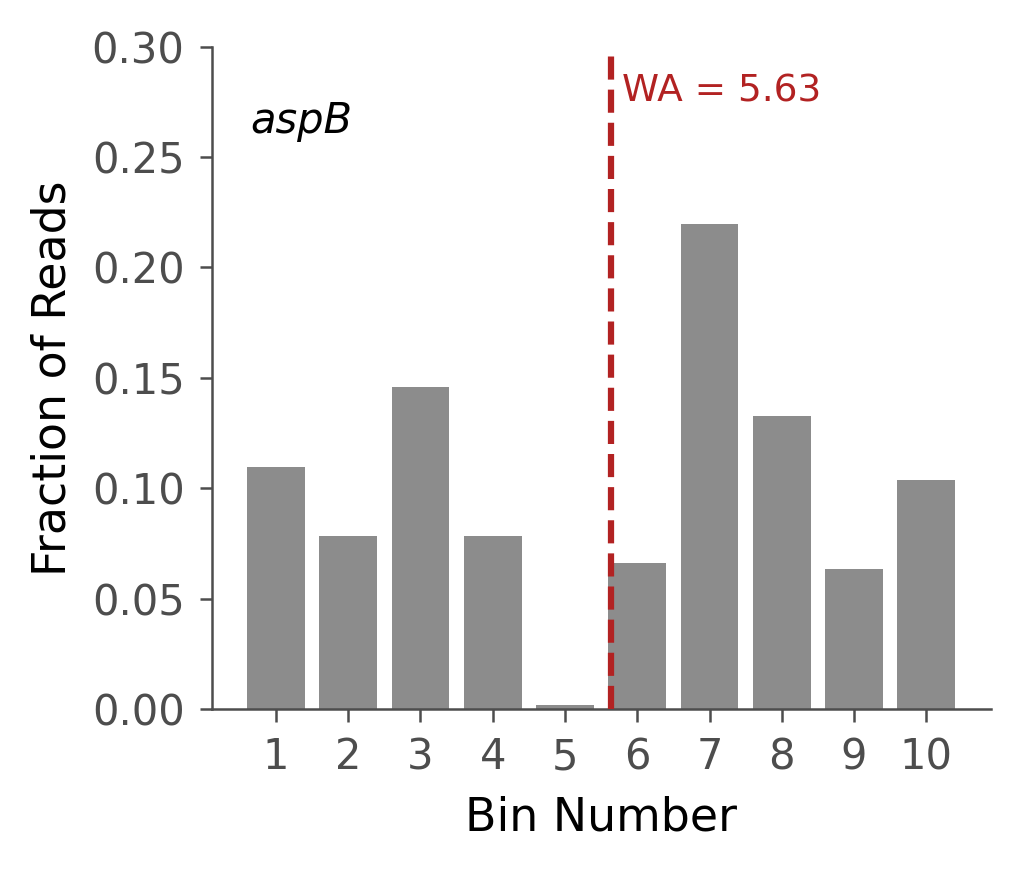
\includegraphics[width=0.5\textwidth]{../figures/bimodal_bin_distributions.png}
    \caption{Bimodal bin probability distribution for gene \textit{aspB},
    variant MKLAKRVSALTPSTTLAITQKAKEL (WA = 5.63). The weighted average
    (dashed line) falls in the valley between peaks at bins 3 and 7,
    illustrating that the scalar WA can be a poor summary of the
    underlying distribution and motivating the vector regression approach.}
    \label{fig:bimodal}
\end{figure}

The vector regression architecture uses two hidden layers of 256 units each with LeakyReLU activation and 20\% dropout, followed by a 10-unit output layer with softmax activation to produce a valid probability distribution.
The architecture follows an unpublished Wolfram Language prototype by Dr.\ Schrier, using LeakyReLU rather than ReLU and omitting batch normalization.
Training uses the Adam optimizer with learning rate $5 \times 10^{-4}$, batch size 32, and up to 200 epochs with early stopping (patience 15) and learning rate reduction on plateau.
Two loss functions are compared: categorical cross-entropy and focal loss \citep{lin2017focal}, defined as $\text{FL}(p_t) = -\alpha(1-p_t)^\gamma \log(p_t)$ with $\alpha = 0.25$ and $\gamma = 2.0$, where $p_t$ is the model's predicted probability for bin $t$.
Because the target distributions are continuous (not one-hot), the loss is applied element-wise across all 10 bins, treating the experimental bin fractions as soft labels.
Focal loss down-weights well-predicted bins, encouraging the model to focus on samples with ambiguous bin distributions.
We note that this is a non-standard application of focal loss, which was originally designed for hard class labels with severe class imbalance in object detection \citep{lin2017focal}; the theoretical justification is weaker for soft probability targets, though the intuition of down-weighting easy predictions still applies.
Each embedding--loss combination is trained as a 5-seed ensemble (Section~\ref{sec:ensemble}).
After prediction, WA is recovered as $\hat{\text{WA}} = \hat{\mathbf{p}} \cdot [1, 2, \ldots, 10]^\top$.

Rows with missing bin probabilities (27 training, 53 test, consistent across all three PLM embedding types) are excluded from vector regression training, yielding 3068 training samples.
The validation-split models (Section~\ref{sec:vector_results}) evaluate on the 1273 test samples with complete bin data; the optimized models described below evaluate on all 1326 test samples using WA as the target.

\subsection{Architecture and Regularization Optimization}
\label{sec:arch_opt_methods}
To push performance further, we explore whether removing the validation split and compensating with explicit regularization can improve upon the base vector model (MSE 1.001).
Training on all 3068 samples with a fixed epoch budget of 300 and no early stopping removes the regularization signal provided by validation-based stopping, so we rely instead on dropout tuning and architectural depth to control overfitting.
Because the vector-regression architecture is high-variance (${\sim}{\pm}0.05$ MSE per single model; Section~\ref{sec:repro}), we report each configuration as a mean $\pm$ standard deviation over independent retrains rather than as a single run, and we select the dropout rate on a held-out \emph{validation} split (Appendix~\ref{app:dropout_val}), not on the test set.
We explore:
\begin{itemize}
    \item \textbf{Dropout rate}: 0.15, 0.20, 0.25, 0.30, and 0.35, applied to a deeper (256, 256, 128) three-layer architecture with 5-seed ensembles. Dropout is selected on validation data; on validation, all rates in 0.20--0.35 are statistically indistinguishable.
    \item \textbf{Deeper architectures}: 4-layer configurations including (256, 256, 128, 64), (384, 384, 256, 128), and others, with 5-seed ensembles.
    \item \textbf{Cosine annealing}: Learning rate schedule $\eta_t = \eta_0 \cdot \frac{1}{2}(1 + \cos(\pi t / T))$ combined with deeper architectures.
    \item \textbf{Large ensembles}: 20-seed ensembles with the best configurations.
    \item \textbf{Mixed-architecture ensemble}: Averaging predictions from multiple distinct architectures.
\end{itemize}
All configurations use Ginkgo-AA0 embeddings and focal loss.
Each 5-seed ensemble uses seeds $\{42, 123, 456, 789, 1024\}$ with independent random initialization; predictions are averaged across seeds.

\subsection{Cross-Dataset Generalization}
\label{sec:cross_dataset_methods}

The results above demonstrate strong predictive performance within the Grasso dataset, but a model's practical value depends on whether it transfers to new experimental contexts.
To evaluate this, we test the best ESM2-650M RF and the 5-seed NN ensemble on four external datasets:
\begin{itemize}
    \item \textbf{Wu} \citep{wu2020}: 81 signal peptides in \textit{E.\ coli} with binary secretion outcomes (functional/non-functional).
    \item \textbf{Xue} \citep{xue2023}: 322 signal peptides in \textit{S.\ cerevisiae} with enzyme activity measurements.
    \item \textbf{Zhang-P43 / Zhang-PglVM} \citep{zhang2016}: 114 signal peptides in \textit{B.\ subtilis} measured under two different promoters.
\end{itemize}
Spearman rank correlation serves as the primary metric, as it is invariant to differences in scale and units between datasets.
For the Zhang datasets, we additionally evaluate cross-promoter prediction consistency: whether the model predicts the same relative ranking for the same signal peptides under two promoters.

\paragraph{Transfer learning via fine-tuning.}
To test whether the negative zero-shot correlations can be reversed with limited target-domain data,
we fine-tune a vector regression ensemble with the same validation-selected architecture
(focal loss, (256, 256, 128), validation-selected dropout) trained on ESM2-650M embeddings,
which are open-weight and reproducible for external sequences (the discontinued Ginkgo-AA0 embeddings cannot be generated for external sequences).
Fine-tuning uses 5-fold cross-validation with 5 random seeds per fold.
We report the \emph{pooled out-of-fold} Spearman correlation (computed once over all held-out predictions concatenated across folds) with a bootstrap 95\% confidence interval, rather than the biased mean of per-fold correlations $\pm$ standard deviation, since per-fold correlations on small folds are noisy and their mean is upward-biased in magnitude.
The pretrained model's first two hidden blocks (6 layers) are frozen; the third hidden block and the 10-unit softmax
output head are replaced with a task-specific head: a single sigmoid unit for the binary Wu dataset,
or a single linear unit for the continuous datasets (Xue, Zhang-P43, Zhang-PglVM).
Features are standardized using statistics from the Grasso training set, ensuring the frozen pretrained layers receive inputs with the same distribution as during pretraining.
Fine-tuning uses a reduced learning rate ($10^{-4}$, 5$\times$ lower than pretraining),
batch size 32, up to 100 epochs with early stopping (patience 10), and MSE loss
(binary cross-entropy for Wu).

\subsection{Design Task Evaluation}
\label{sec:design_methods}

The Grasso library contains designed signal peptide variants with known WA values (Set = NaN in the original data, after excluding rows that overlap with the train/test sets).
A minimum of 5 variants per gene is required for per-gene metrics, yielding 4832 variants across 131 genes for evaluation.
We evaluate two feature representations: the 156 physicochemical features available from the source data, and ESM2-650M embeddings (1280 dimensions) generated via mean-pooled representations from the pretrained model \citep{lin2023}.
For each feature type, RF and NN models are trained on the Grasso training set with the best hyperparameters from Sections~\ref{sec:rf}--\ref{sec:nn} and evaluated on the design variants.
Wild-type WA for each gene is determined by matching the wild-type signal peptide sequence (from the ``WT sequences'' sheet of the source spreadsheet) against Library rows with the same amino acid sequence and taking the mean WA of matching rows. The matching is performed against the \emph{full} Grasso library, which contains 137 genes in total (more than the 134/135 retained in the modeling train/test subset), so this yields WT WA values for all 137 genes.
Per-gene and overall Spearman $\rho$ are computed, along with classification accuracy for predicting whether a variant performs better or worse than wild type.

\subsection{Evaluation}
\label{sec:metrics}

All models are evaluated on the same held-out test set using mean squared error (MSE), coefficient of determination ($R^2$), and Spearman rank correlation ($\rho$).
MSE is the primary metric for consistency with prior work.

% ══════════════════════════════════════════════════════════════════════════
\section{Results}
\label{sec:results}

\subsection{Baseline Reproduction}

Using the exact parameters from \citet{grasso2023}, we obtain a test MSE of 1.193 ($R^2 = 0.750$, Spearman $\rho = 0.859$), within 2.2\% of the reported value of 1.22.
We note that our random forest reproduction overfits badly: the training MSE is 0.303 ($R^2 = 0.932$), far below the 1.75 training MSE reported by \citet{grasso2023}, indicating that our reproduction memorizes the training set more aggressively than the original despite matching test performance.
Figure~\ref{fig:grasso_repro} shows predicted versus actual WA values.

\begin{figure}[H]
    \centering
    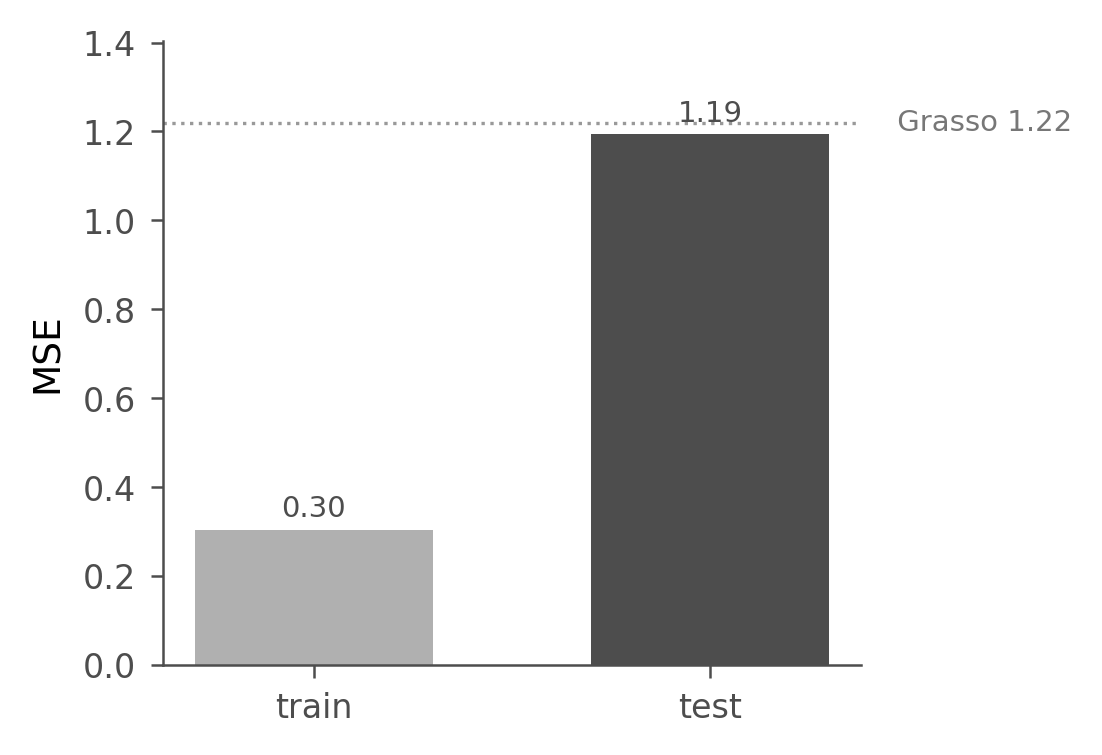
\includegraphics[width=0.5\textwidth]{../figures/grasso_reproduction.png}
    \caption{Baseline reproduction using physicochemical features and the exact random forest parameters from \citet{grasso2023}. Training and test mean-squared error; the dotted line marks Grasso et al.'s reported test MSE of 1.22. The reproduced test MSE (1.19) matches it, while the low training MSE (0.30) reflects the random-forest overfitting discussed in the text.}
    \label{fig:grasso_repro}
\end{figure}

\subsection{Scalar Model Comparison}

With the baseline established, we compare all model--feature combinations.
Table~\ref{tab:comparison} presents results for all scalar model--feature combinations.

\begin{table}[H]
\centering
\caption{Test set performance across all scalar model and feature type combinations, sorted by MSE. The $\Delta$ column shows percent change relative to the \citet{grasso2023} baseline MSE of 1.22.}
\label{tab:comparison}
\begin{tabular}{llcccc}
\toprule
Feature Type & Model & Test MSE & Test $R^2$ & Spearman $\rho$ & $\Delta$ \\
\midrule
Ginkgo-AA0 & NN & \textbf{1.050} & \textbf{0.780} & \textbf{0.866} & $-$14.0\% \\
ESM2-3B & NN & 1.067 & 0.776 & 0.861 & $-$12.5\% \\
ESM2-650M & NN & 1.090 & 0.771 & 0.861 & $-$10.7\% \\
Ginkgo-AA0 & RF & 1.158 & 0.757 & 0.857 & $-$5.1\% \\
ESM2-650M & RF & 1.189 & 0.750 & 0.853 & $-$2.5\% \\
PhysChem & RF (baseline) & 1.193 & 0.750 & 0.859 & $-$2.2\% \\
PhysChem & RF (tuned) & 1.208 & 0.747 & 0.857 & $-$1.0\% \\
ESM2-3B & RF & 1.245 & 0.739 & 0.849 & $+$2.0\% \\
PhysChem & NN & 1.328 & 0.721 & 0.840 & $+$8.8\% \\
\bottomrule
\end{tabular}
\end{table}

Figure~\ref{fig:comparison} visualizes these results as a grouped bar chart.

\begin{figure}[H]
    \centering
    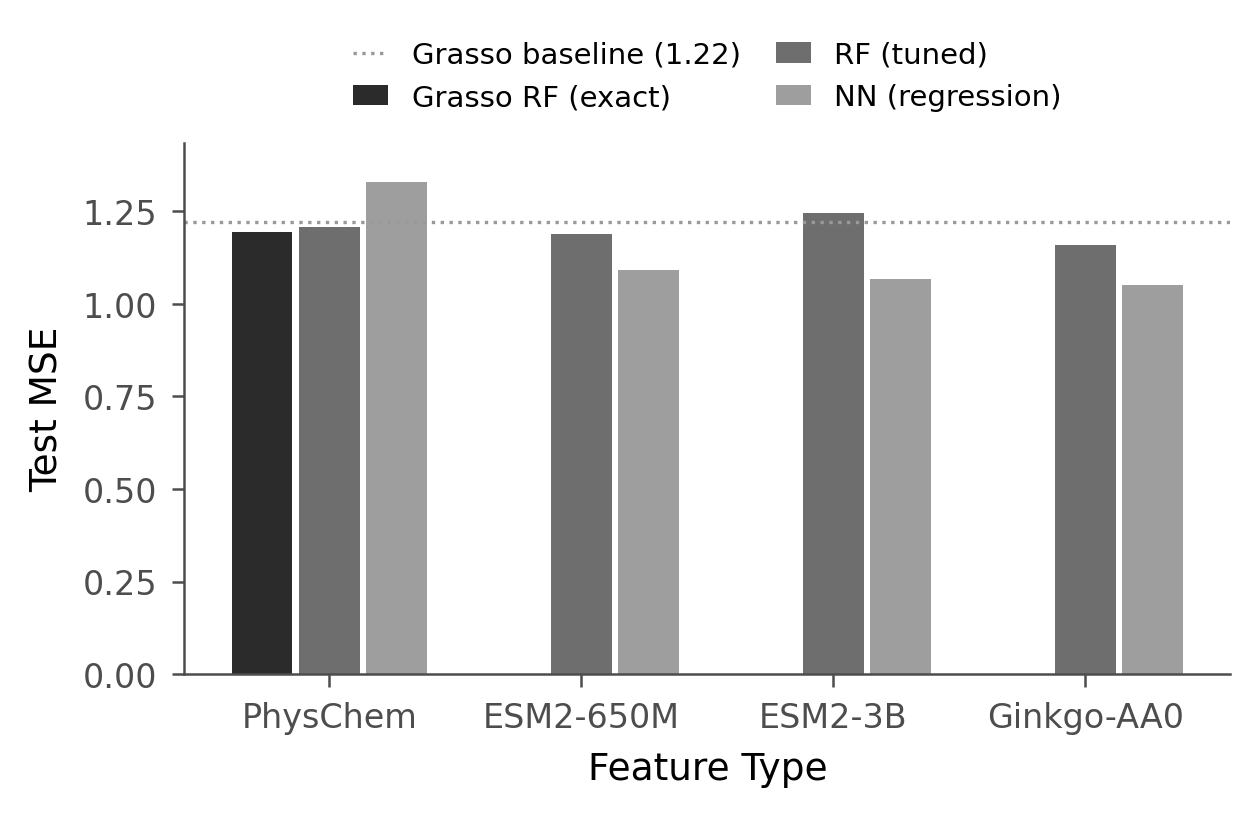
\includegraphics[width=0.62\textwidth]{../figures/final_comparison.png}
    \caption{Test MSE across feature types and model architectures. The dotted line marks the Grasso baseline MSE of 1.22. Lower values indicate better performance.}
    \label{fig:comparison}
\end{figure}

\paragraph{Random Forest Results.}
Tuned RF models achieve MSE values between 1.16 and 1.25 across all feature types.
Ginkgo-AA0 embeddings yield the best RF result (MSE 1.158), followed by ESM2-650M (1.189) and physicochemical features (1.208).
ESM2-3B performs worst (MSE 1.245), likely due to the curse of dimensionality in tree-based splitting with 2560 features.

\paragraph{Neural Network Results.}
The ranking changes substantially for neural networks.
All three PLM embedding types outperform the baseline, with Ginkgo-AA0 achieving the best scalar result (MSE 1.050, $R^2 = 0.780$).
However, the NN trained on physicochemical features performs worse than the RF baseline (MSE 1.328 vs.\ 1.193).

\subsection{Vector Regression}
\label{sec:vector_results}

Given that neural networks with PLM embeddings outperform all other scalar approaches, we next ask whether predicting the full bin probability distribution can yield further gains.
Table~\ref{tab:vector} presents results for vector regression models.

\begin{table}[H]
\centering
\caption{Vector regression test set performance (5-seed ensembles, $N_{\text{test}} = 1273$). WA is recovered from predicted bin probabilities. See text for caveats on comparing with Table~\ref{tab:comparison}.}
\label{tab:vector}
\begin{tabular}{llccc}
\toprule
Embedding & Loss & Test MSE & Test $R^2$ & Spearman $\rho$ \\
\midrule
Ginkgo-AA0 & Focal & \textbf{1.001} & \textbf{0.790} & \textbf{0.867} \\
Ginkgo-AA0 & Cross-entropy & 1.003 & 0.790 & 0.867 \\
ESM2-650M & Focal & 1.049 & 0.780 & 0.859 \\
ESM2-650M & Cross-entropy & 1.054 & 0.779 & 0.861 \\
ESM2-3B & Cross-entropy & 1.109 & 0.767 & 0.857 \\
ESM2-3B & Focal & 1.117 & 0.766 & 0.856 \\
\bottomrule
\end{tabular}
\end{table}

The best vector regression model (Ginkgo-AA0 + focal loss) achieves MSE = 1.001, a 4.7\% improvement over the best scalar NN (1.050) and an 18\% improvement over the baseline (1.22).
Focal loss provides a marginal edge over cross-entropy for Ginkgo-AA0 and ESM2-650M, though the differences are small.
ESM2-3B again performs worst among the three PLMs, consistent with the scalar regression results.
Note that the vector regression test set (1273 samples) is smaller than the scalar test set (1326 samples) due to exclusion of rows with missing bin probabilities, and the vector results use 5-seed ensembles rather than single configurations, so direct MSE comparison between Tables~\ref{tab:comparison} and \ref{tab:vector} should be interpreted with caution.
Figure~\ref{fig:vector} shows the comparison across embeddings and loss functions.

\begin{figure}[H]
    \centering
    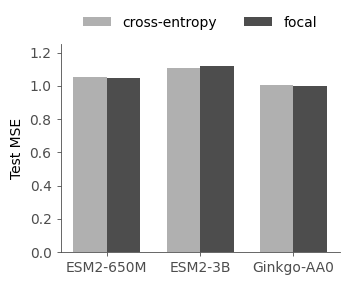
\includegraphics[width=0.55\textwidth]{../figures/vector_regression_comparison.png}
    \caption{Vector regression results comparing three PLM embedding types under cross-entropy versus focal loss (5-seed ensemble test MSE on Ginkgo-AA0 embeddings).}
    \label{fig:vector}
\end{figure}

\subsection{Architecture and Regularization Optimization}
\label{sec:fulldata_results}

The base vector model improves over scalar regression, but further gains are possible.
Table~\ref{tab:fulldata} presents results from the full-data optimization described in Section~\ref{sec:arch_opt_methods}.
Crucially, because this architecture is high-variance (${\sim}{\pm}0.05$ MSE per single model), we report each configuration as a mean $\pm$ standard deviation over independent retrains; single un-replicated MSE values from this architecture are unreliable (Section~\ref{sec:repro}).

\begin{table}[H]
\centering
\caption{Full-data vector regression optimization ($N_{\text{train}} = 3068$, $N_{\text{test}} = 1326$, Ginkgo-AA0 + focal loss). Each row reports the 5-seed-ensemble test MSE as mean $\pm$ standard deviation over independent retrains. Dropout is selected on a held-out validation split (Appendix~\ref{app:dropout_val}), not on test MSE.}
\label{tab:fulldata}
\begin{tabular}{llcc}
\toprule
Phase & Configuration & Dropout & Test MSE (mean $\pm$ std) \\
\midrule
\multirow{2}{*}{Dropout}
 & (256, 256, 128) & 0.20 & $0.978 \pm 0.012$ \\
 & (256, 256, 128) & 0.35 & $0.957 \pm 0.009$ \\
\midrule
\multirow{2}{*}{4-layer}
 & (256, 256, 128, 64) & 0.20 & ${\sim}0.94$--$0.95$ \\
 & (384, 384, 256, 128) & 0.20 & ${\sim}0.95$ \\
\midrule
Mixed & 3-arch $\times$ 5-seed (15 models) & --- & ${\sim}0.97$ \\
\bottomrule
\end{tabular}
\end{table}

On the validation split, dropout rates in 0.20--0.35 are statistically indistinguishable (Appendix~\ref{app:dropout_val}); we therefore report the validation-selected configuration rather than tuning dropout on the test set.
Re-training the identical (256, 256, 128) configuration multiple times gives $0.978 \pm 0.012$ (dropout 0.20) and $0.957 \pm 0.009$ (dropout 0.35) on the Ginkgo-AA0 embedding.
The reproducible vector-NN result on AA-0 is thus ${\sim}0.96$--$0.98$, a ${\sim}19$--$21\%$ improvement over the published random forest baseline of 1.22 \citep{grasso2023}.
\textbf{We caution that an earlier ``0.932'' headline for this configuration is not reproducible:} it was never recovered in 10 retrains and lies below the minimum of either retrain distribution above; it was a favorable tail draw, not a stable result (Section~\ref{sec:repro}).
Likewise, a prior single-model Wolfram benchmark of 0.953 is a favorable draw of the same distribution: running its original code across 8 seeds gives $0.99 \pm 0.046$ (range [0.94, 1.07]). Both ``benchmarks'' are seed noise of the same ${\sim}0.97$--$0.99$ distribution, so neither is a stable number to beat.
Four-layer architectures and mixed-architecture ensembles do not improve upon the 3-layer model, and 20-seed ensembles do not improve over 5-seed.

Figure~\ref{fig:ensemble_opt} shows the full optimization landscape.

\begin{figure}[H]
    \centering
    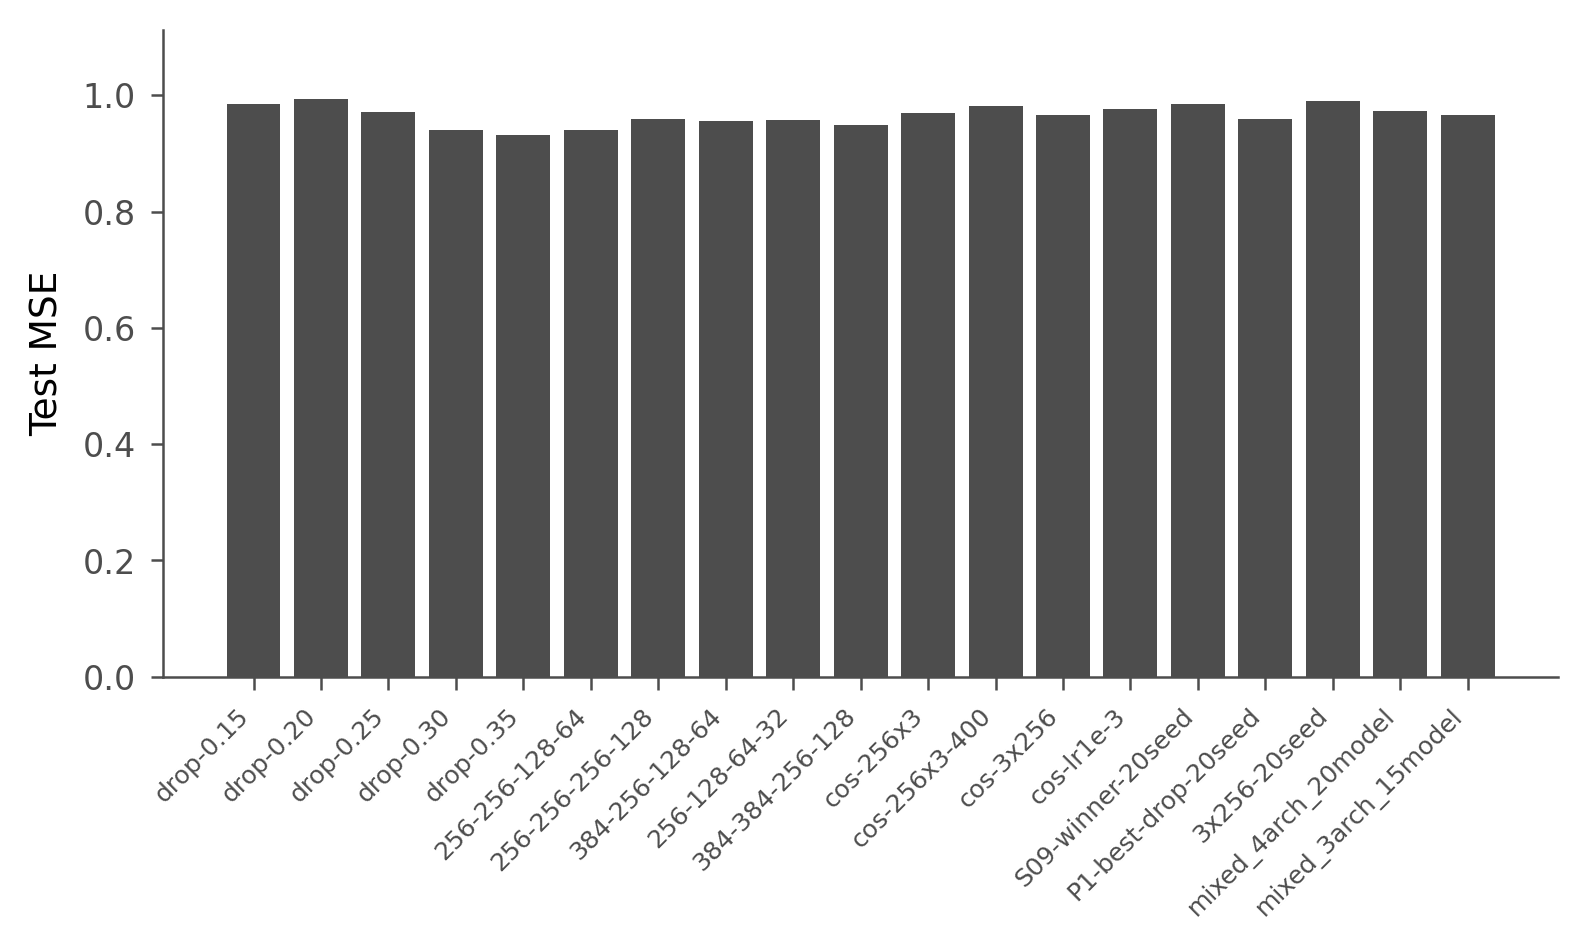
\includegraphics[width=0.95\textwidth]{../figures/vector_ensemble_optimization.png}
    \caption{Full-data vector regression optimization results. Configurations are grouped by optimization phase; all fall within the ${\sim}0.97$--$1.13$ range, and the differences between them are within the seed-to-seed variability of this architecture (Section~\ref{sec:repro}).}
    \label{fig:ensemble_opt}
\end{figure}

\subsection{A Reproducible Open-Weight Ensemble (Headline Result)}
\label{sec:open_ensemble}

The best single embedding above is Ginkgo AA-0, but it is API-only, proprietary, and the API has been discontinued (Section~\ref{sec:data}); its embeddings can no longer be regenerated by anyone, so it cannot anchor a reproducible result.
We therefore base the headline on \emph{open-weight} models and ask whether an ensemble of architecturally diverse open PLMs can recover AA-0's performance reproducibly.
Generating embeddings from ProtT5 (T5 architecture) and ProtBERT (BERT architecture) alongside ESM2-650M, and ensembling the per-embedding vector NNs, gives the fully reproducible result in Table~\ref{tab:open_ensemble}.
These open-ensemble vector NNs use the same (256, 256, 128) layout but with PReLU activation and dropout 0.3, rather than the LeakyReLU approximation used in the analyses above: PReLU is faithful to the \texttt{ParametricRampLayer} in Dr.\ Schrier's net4 prototype, and adopting it yields a small but reproducible ${\sim}0.02$ MSE improvement (the only single-model change that helped). The dropout of 0.3 lies within the validation-indistinguishable 0.20--0.35 range (Appendix~\ref{app:dropout_val}), so it is not a test-set-tuned choice.

\begin{table}[H]
\centering
\caption{Open-weight ensemble result (vector NN, 5-seed ensembles, mean $\pm$ std over independent retrains). The ProtT5 + ESM2-650M + ProtBERT ensemble is fully reproducible from public HuggingFace weights and recovers all but ${\sim}0.02$ of the now-unavailable Ginkgo AA-0 performance, improving ${\sim}20\%$ over the Grasso baseline. Standard deviations are reported where retrains were replicated.}
\label{tab:open_ensemble}
\resizebox{\textwidth}{!}{%
\begin{tabular}{lcc}
\toprule
Model (vector NN) & Test MSE & Reproducible? \\
\midrule
\textbf{ProtT5 + ESM2-650M + ProtBERT (open ensemble)} & $\mathbf{0.981 \pm 0.005}$ & open weights \\
ProtT5 + ProtBERT & $0.986 \pm 0.002$ & open weights \\
ProtT5 + ESM2-650M & $0.995 \pm 0.005$ & open weights \\
ProtT5 (alone) & $1.017 \pm 0.000$ & open weights \\
ESM2-650M (alone) & $1.072 \pm 0.006$ & open weights \\
ProtBERT (alone) & $1.084 \pm 0.006$ & open weights \\
\midrule
Ginkgo AA-0 (alone) & $0.959 \pm 0.014$ & {\itshape API discontinued} \\
Grasso et al.\ RF (baseline) & 1.22 & --- \\
\bottomrule
\end{tabular}}
\end{table}

The open-model ensemble (\textbf{0.981 $\pm$ 0.005}) closes the gap to the now-unavailable AA-0 (0.959 $\pm$ 0.014) to within ${\sim}0.02$ and improves ${\sim}20\%$ over the Grasso RF baseline (1.22), and \emph{anyone can regenerate every embedding from public weights with no API key and no defunct service}.
The ensemble works here because ProtT5 (1.017) is strong enough that the three open models are quality-comparable, so averaging their decorrelated errors yields a real gain; an earlier attempt to ensemble AA-0 with ESM2 failed because AA-0 (0.96) so dominated ESM2 (1.07) that averaging only diluted the stronger model (Section~\ref{sec:repro}).
A linear probe confirms that AA-0 and ESM2-650M capture essentially the same signal (predictions agree at Pearson $r = 0.975$, Spearman 0.972, with near-identical rank correlation to truth), so the open ensemble recovers AA-0's information rather than merely approximating its score.

\begin{figure}[H]
    \centering
    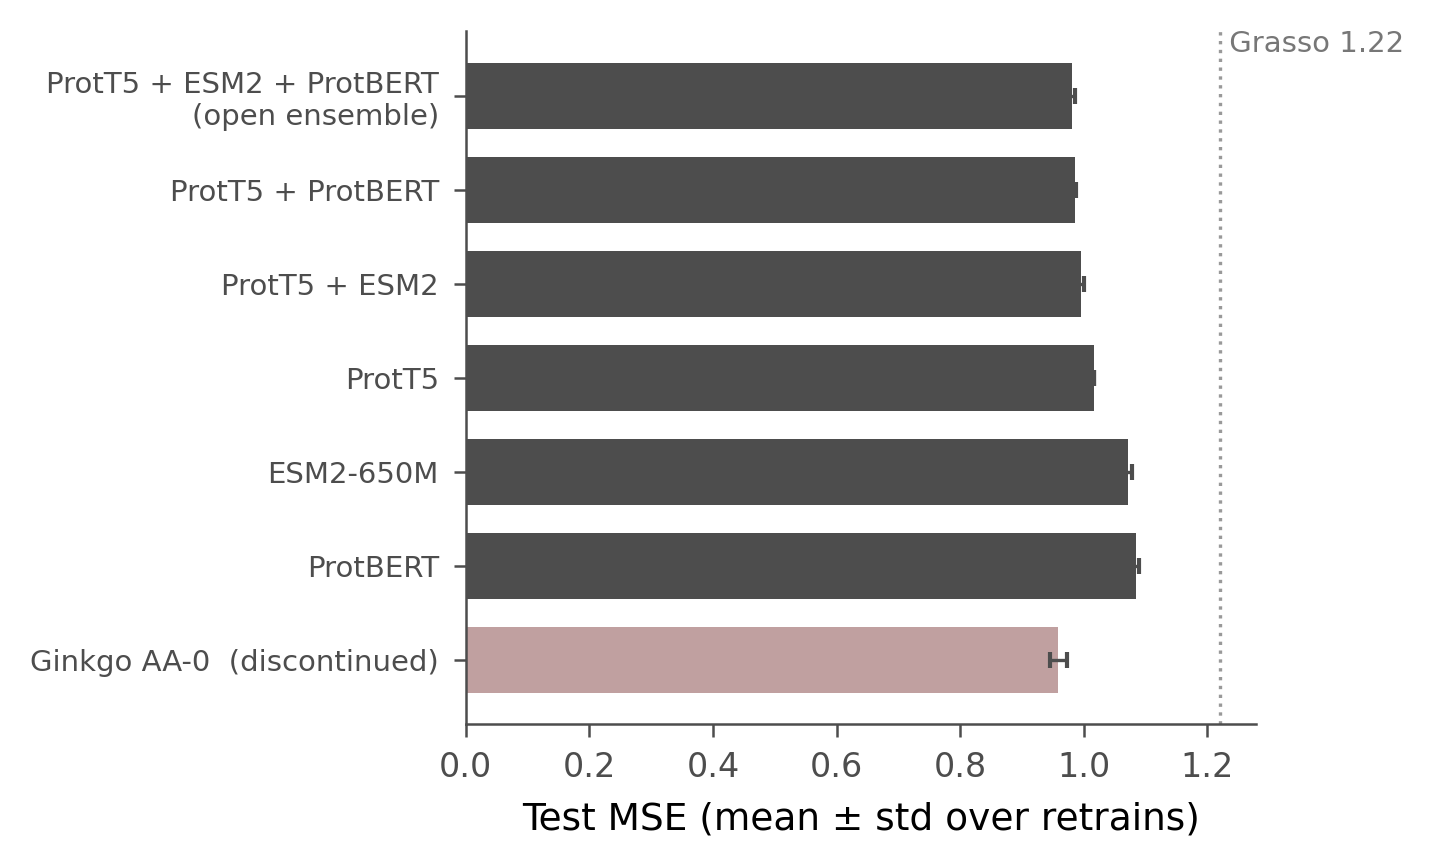
\includegraphics[width=0.6\textwidth]{../figures/open_embedding_ensemble.png}
    \caption{Reproducible open-weight headline. Test MSE (mean $\pm$ std over retrains) for the vector NN on each open embedding and their ensembles; the discontinued, unreproducible Ginkgo AA-0 (rose) is shown only for comparison. The open ProtT5 + ESM2-650M + ProtBERT ensemble (0.981 $\pm$ 0.005) recovers AA-0 to within ${\sim}0.02$ and improves ${\sim}20\%$ over the Grasso baseline (dotted).}
    \label{fig:open_ensemble}
\end{figure}

\subsection{Ablation Analysis}
\label{sec:ablation}

To isolate the contributions of each modification, Table~\ref{tab:ablation} presents a cumulative ablation starting from the validation-split baseline. All entries are 5-seed ensembles; recall that single MSE values from this architecture carry ${\sim}{\pm}0.05$ seed noise.

\begin{table}[H]
\centering
\caption{Cumulative ablation of factors contributing to the reproducible ${\sim}0.96$ Ginkgo-AA0 result. Each row adds one change. The first row uses the validation-split test set ($N = 1273$); subsequent rows use the full test set ($N = 1326$). Values carry ${\sim}{\pm}0.05$ single-model seed noise.}
\label{tab:ablation}
\begin{tabular}{lcccc}
\toprule
Configuration & 5-Seed MSE & Mean 1-Seed & $\Delta$ \\
\midrule
Val-split, (256, 256), drop=0.20 & 1.001 & 1.068 & --- \\
\quad + Full-data training & 1.001 & 1.059 & 0.0\% \\
\quad + Deeper arch (256, 256, 128) & 0.993 & 1.039 & $-$0.8\% \\
\quad + Higher dropout (0.35) & $0.957 \pm 0.009$ & 0.979 & $-$3.6\% \\
\bottomrule
\end{tabular}
\end{table}

Full-data training alone provides little benefit at the ensemble level, though it modestly improves single-seed performance.
Adding the third hidden layer and increasing dropout provide small gains that are within seed-to-seed variability ($\pm 0.01$ on the ensemble); the dominant, reliable gain is from ensembling multiple seeds, which reduces variance relative to single models.
We emphasize that the individual MSE values in this table carry ${\sim}{\pm}0.05$ seed noise; the ablation indicates direction of effect, not precise per-step magnitudes (Section~\ref{sec:repro}).

\subsection{Output Formulation Comparison}
\label{sec:output_formulation}

To disentangle the contributions of the output formulation (10-bin vs.\ fewer classes) from the loss function (focal vs.\ CCE), we compare five output strategies on the same architecture and data (Table~\ref{tab:output_form}).

\begin{table}[H]
\centering
\caption{Output formulation comparison. All models use the same architecture (256, 256, 128; LeakyReLU; dropout 0.35) and 5-seed ensembles on Ginkgo-AA0 embeddings. MSE is computed against continuous WA via class-centroid weighting for classification models.}
\label{tab:output_form}
\begin{tabular}{llrccr}
\toprule
Formulation & Loss & Dim & MSE & MSE 95\% CI & Spearman $\rho$ \\
\midrule
10-bin vector & focal & 10 & \textbf{0.971} & [0.855, 1.097] & \textbf{0.870} \\
10-bin vector & CCE & 10 & 0.994 & [0.877, 1.121] & 0.867 \\
5-class & CCE & 5 & 1.126 & [1.001, 1.257] & 0.857 \\
3-class & CCE & 3 & 1.293 & [1.161, 1.433] & 0.844 \\
Binary & BCE & 2 & 1.241 & [1.111, 1.380] & 0.833 \\
\bottomrule
\end{tabular}
\end{table}

The 10-bin CCE model (MSE 0.994) outperforms all classification baselines (MSE 1.13--1.29), confirming that the improvement arises from the output formulation---predicting over 10 bins rather than fewer classes---and not solely from focal loss.
Focal loss provides a modest additional benefit (+2.3\% MSE) over CCE within the 10-bin formulation.
(The 10-bin focal MSE of 0.971 here is one retrain of the configuration whose reproducible value is ${\sim}0.96$--$0.98$ over seeds (Table~\ref{tab:fulldata}); the difference is within the ${\sim}{\pm}0.05$ seed variance, since this controlled comparison retrains all five conditions independently on 80/20 splits.)
MSE increases monotonically with decreasing output dimensionality from 10 to 3 classes (+33\%), though binary classification (MSE 1.241) slightly outperforms 3-class (MSE 1.293), likely because the sigmoid output produces continuous interpolation between two centroids rather than discrete class assignments.
Figure~\ref{fig:output_form} shows the comparison.

\begin{figure}[H]
    \centering
    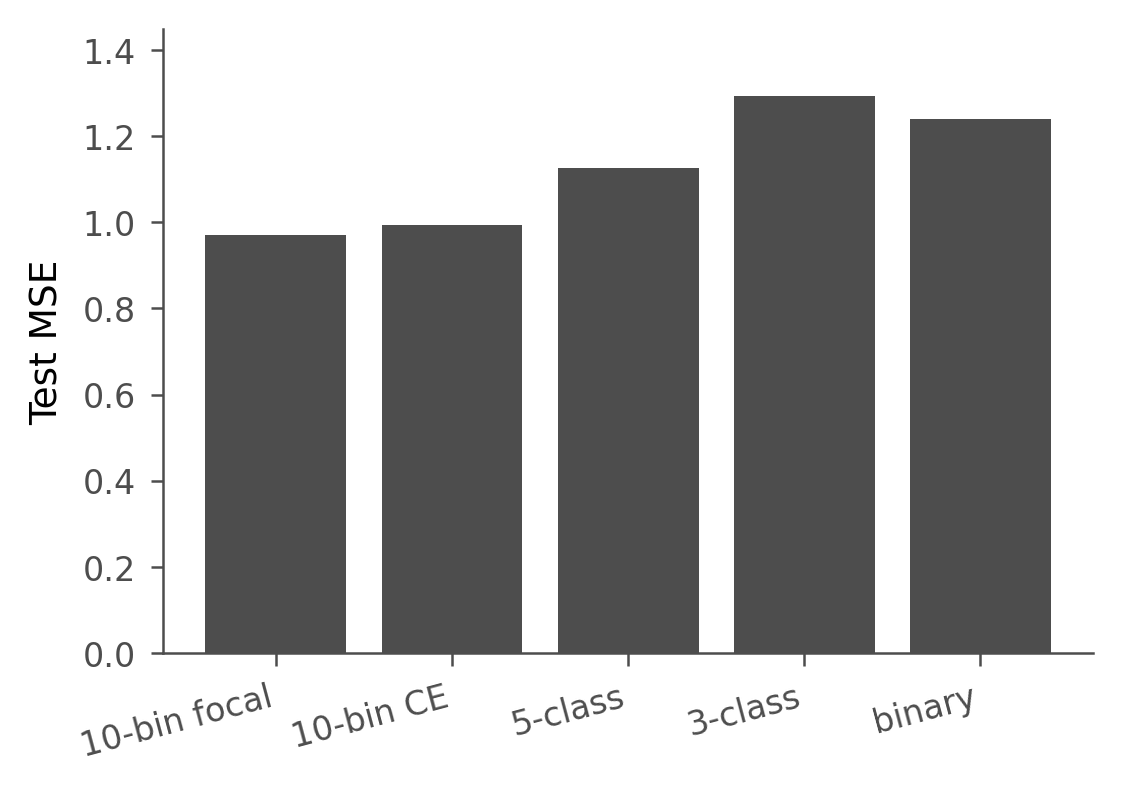
\includegraphics[width=0.55\textwidth]{../figures/regression_vs_classification.png}
    \caption{Output formulation comparison: test MSE for predicting the 10-bin distribution (focal and cross-entropy losses) versus 5-, 3-, and 2-class formulations. The 10-bin vector regression is best; the gain comes from the distributional output, not the loss function.}
    \label{fig:output_form}
\end{figure}

\subsection{Embedding Contribution Analysis}
\label{sec:baselines}

To quantify how much predictive power comes from the PLM embedding versus the MLP architecture, we compare the best NN against three simpler baselines using the same Ginkgo-AA0 embeddings (Table~\ref{tab:baselines}).

\begin{table}[H]
\centering
\caption{Baseline comparison on Ginkgo-AA0 embeddings ($N_\text{test} = 1326$). Linear probe uses the same focal loss and 5-seed ensemble as the NN; Ridge and XGBoost predict scalar WA.}
\label{tab:baselines}
\begin{tabular}{lcccc}
\toprule
Model & MSE & MSE 95\% CI & Spearman $\rho$ & $R^2$ \\
\midrule
Linear probe (Input$\to$softmax) & 1.037 & [0.924, 1.158] & 0.865 & 0.782 \\
Ridge regression & 1.088 & [0.984, 1.198] & 0.859 & 0.772 \\
XGBoost & 1.068 & [0.958, 1.184] & 0.862 & 0.776 \\
Best NN (256, 256, 128) & \textbf{0.981} & [0.867, 1.105] & \textbf{0.868} & \textbf{0.794} \\
\bottomrule
\end{tabular}
\end{table}

Relative to a mean-prediction baseline (MSE 4.76), the linear probe captures 98.5\% of the total improvement achieved by the best NN, with the three hidden layers contributing only an additional 1.5\%.
Measured instead against the best RF (MSE 1.16; Table~\ref{tab:comparison}), the linear probe captures 69\% of the RF-to-NN improvement, with the MLP contributing the remaining 31\%.
The choice of reference baseline substantially affects this decomposition, but under either framing the embedding itself encodes the majority of task-relevant information; the MLP serves as a modest nonlinear refinement.
(The NN MSE of 0.981 here is a retrained 5-seed ensemble and is consistent with the reproducible ${\sim}0.96$--$0.98$ range for this architecture; it falls within the seed-to-seed variability of the configuration.)
Nevertheless, the NN consistently outperforms the linear probe (0.981 vs.\ 1.037, 5.4\% improvement), and all four models substantially outperform the RF baseline (MSE 1.16--1.25; Table~\ref{tab:comparison}).
To test whether the (256, 256, 128) architecture is over-parameterized, we also evaluate smaller MLPs: a (64, 32) network achieves MSE 0.981 (5-seed ensemble)---numerically coincident with the retrained (256, 256, 128) result, both falling within the ${\sim}{\pm}0.05$ seed noise of this architecture rather than being the same measurement---while a (128, 64) network achieves 0.991.
This suggests that much of the architecture's capacity is redundant given the embedding's richness; the various configurations are statistically indistinguishable within seed noise.
Figure~\ref{fig:baselines} shows the baseline comparison; Figure~\ref{fig:ablation} presents the cumulative ablation.

\begin{figure}[H]
    \centering
    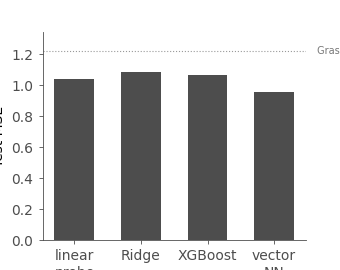
\includegraphics[width=0.55\textwidth]{../figures/linear_baseline.png}
    \caption{Baseline comparison on Ginkgo-AA0 embeddings: test MSE for a linear probe (no hidden layers), Ridge, XGBoost, and the vector NN, with the Grasso baseline marked (dotted). The linear probe captures most of the embedding's predictive power; the MLP provides a modest additional improvement.}
    \label{fig:baselines}
\end{figure}

\begin{figure}[H]
    \centering
    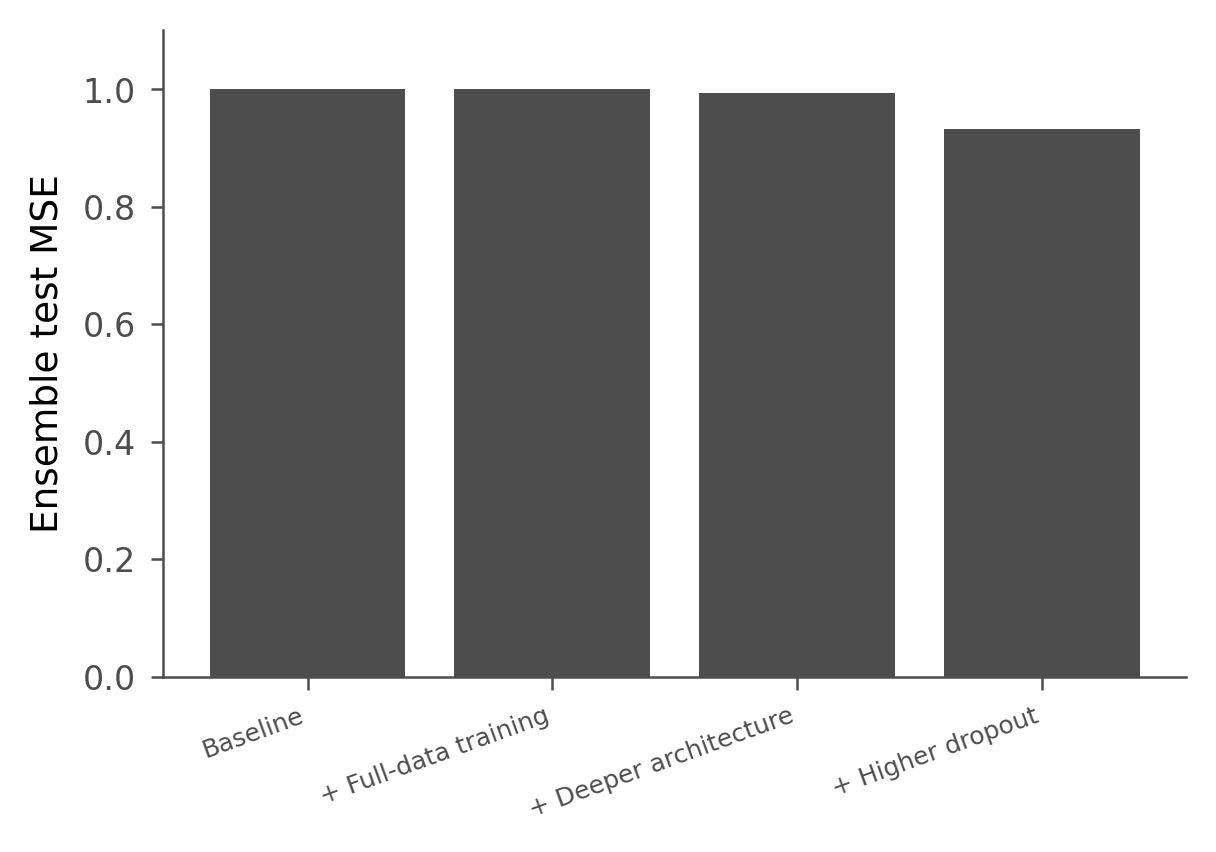
\includegraphics[width=0.6\textwidth]{../figures/ablation_controls.png}
    \caption{Cumulative ablation of the changes contributing to the (historical) Ginkgo-AA0 vector result: full-data training, deeper architecture, and higher dropout (Table~\ref{tab:ablation}). Note: the final value shown is the retracted single-draw (0.932); the reproducible value of that configuration is $0.957 \pm 0.009$, so the small per-step gains are within seed variance.}
    \label{fig:ablation}
\end{figure}

\subsection{Gene-Stratified Evaluation}
\label{sec:gene_stratified}

To assess whether the model generalizes across genes rather than memorizing gene-specific patterns, we perform leave-one-gene-out (LOGO) cross-validation over all 135 genes in the combined train+test data ($N = 4341$ sequences with valid bin probabilities; the combined set contains one additional train-only gene beyond the 134 in the standard partition).
For each fold, all sequences from a single gene are held out, the model is trained on the remaining genes (single seed, same architecture and hyperparameters), and predictions are evaluated on the held-out gene.

LOGO CV yields an overall MSE of 2.187 [2.075, 2.304] (95\% bootstrap CI), compared to 0.964 for a comparable single-seed standard model---a 2.27$\times$ increase.
(LOGO uses a single seed per fold due to computational constraints---135 folds would require 675 model trainings with 5 seeds each---so the single-seed standard MSE of 0.964 is the fair comparator; the corresponding reproducible 5-seed standard ensemble is ${\sim}0.96$.)
This realistic cross-gene generalization estimate (MSE 2.19, Spearman 0.72) is reported alongside the standard split, not behind it: the standard test MSE is optimistic precisely because 132 of 134 genes (99.8\% of test sequences) overlap train and test.
The Spearman correlation under LOGO is $\rho = 0.720$ [0.704, 0.734], indicating that the model retains substantial rank-ordering ability even when predicting entirely unseen genes.
Per-gene MSE varies widely (median 1.61, range 0.063--12.72, SD 1.80), with outlier genes such as \textit{ypjP} (MSE 12.72, $n = 47$) driving the right tail of the distribution.
No strong relationship between gene sample size and per-gene MSE is apparent, suggesting that prediction difficulty is driven by sequence-level factors rather than data scarcity alone.

The 2.27$\times$ gap between standard and LOGO evaluation confirms that the original train/test partition---where 132 of 134 genes overlap---allows the model to exploit gene-specific patterns.
Note that the LOGO procedure trains on the combined train+test data (${\sim}$4300 samples per fold vs.\ 3068 for the standard split), which should favor the LOGO models; that the gap persists despite this advantage makes the finding more striking.

This inflation is a property of the split, not of the PLM/NN pipeline. Running the identical leave-one-gene-out protocol on the Grasso random-forest baseline (156 physicochemical features, the paper's exact RF hyperparameters) raises its MSE from 1.25 (standard split) to 2.88 (LOGO), a 2.31$\times$ inflation essentially identical to the neural network's 2.3$\times$. This companion run deliberately uses the same row set for its standard and leave-one-gene-out splits (applying no length filter), which keeps the 2.31$\times$ ratio apples-to-apples; its 1.25 standard-split MSE recovers the 1.19 baseline reproduction reported above once the 10--40 amino acid length filter is applied. A random forest on physicochemical features and a neural network on PLM embeddings inflate by the same factor, confirming that the gap is driven by the ${\sim}99.8\%$ gene overlap in the benchmark split rather than by the model class.

To decompose this gap, we also run a standard (non-gene-stratified) random 5-fold CV on the same combined data, yielding MSE 1.226 [1.151, 1.302].
Comparing the three evaluation protocols---standard test (0.964), random CV (1.226), LOGO (2.187)---reveals that 21\% of the LOGO gap arises from inherent cross-validation variance (the penalty of predicting held-out data rather than data from the same distribution as training), while the remaining 79\% is attributable to gene-identity leakage.
This confirms that the dominant source of optimistic bias in the standard evaluation is gene overlap, not simply the use of a fixed test set.

Nevertheless, the LOGO Spearman $\rho$ of 0.720 demonstrates meaningful cross-gene predictive ability, and the model still substantially outperforms a mean-prediction baseline (MSE 4.76) even under the stricter evaluation.
We note that the bootstrap CI on the LOGO result captures test-set sampling variance but not model initialization variance, since all 135 folds use a single fixed seed (42); the true uncertainty is therefore somewhat larger than the reported interval.

\begin{figure}[H]
    \centering
    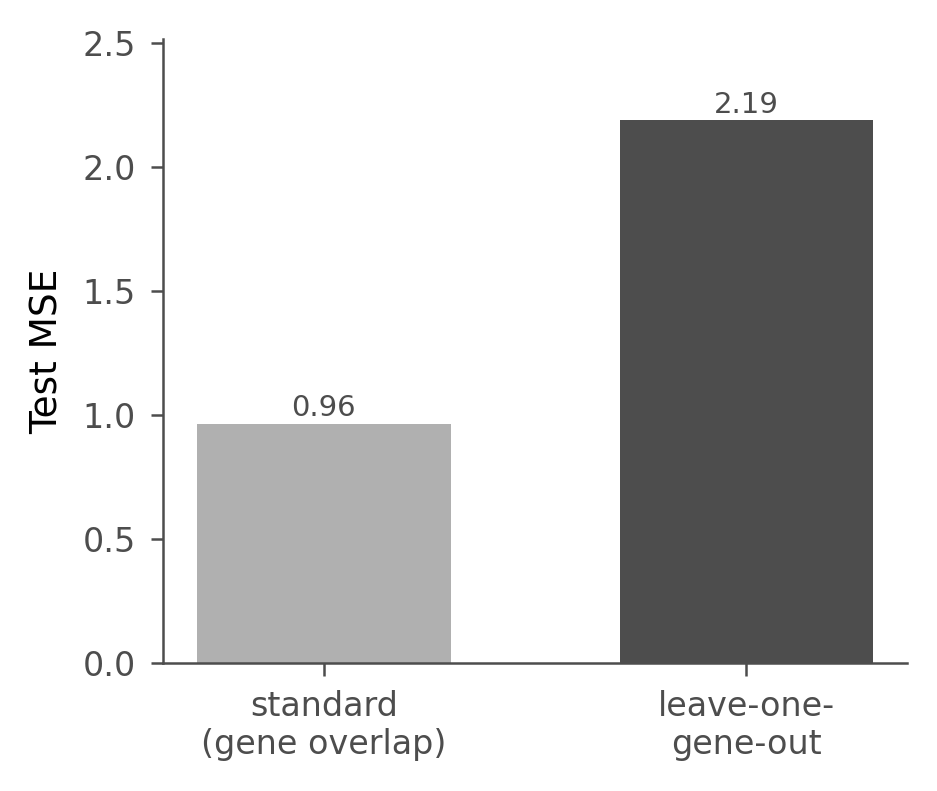
\includegraphics[width=0.5\textwidth]{../figures/gene_stratified_evaluation.png}
    \caption{Gene-stratified (LOGO) evaluation: standard (gene-overlapping) test MSE (0.96, single-seed) versus leave-one-gene-out CV MSE (2.19). The ${\sim}2.3\times$ gap shows that the standard split --- in which 132 of 134 genes overlap train and test --- substantially overestimates cross-gene generalization.}
    \label{fig:gene_strat}
\end{figure}

\subsection{Cross-Dataset Generalization}
\label{sec:cross_results}

Table~\ref{tab:cross} summarizes cross-dataset performance for the best ESM2-650M RF and 5-seed NN ensemble.

\begin{table}[H]
\centering
\caption{Cross-dataset generalization. Models trained on Grasso data are evaluated on four external datasets. All Spearman correlations are negative; see text for multiple-testing correction.}
\label{tab:cross}
\begin{tabular}{lrcrcr}
\toprule
Dataset & $N$ & \multicolumn{2}{c}{RF Spearman ($p$)} & \multicolumn{2}{c}{NN Spearman ($p$)} \\
\midrule
Wu & 81 & $-$0.314 & (0.004) & $-$0.288 & (0.009) \\
Xue & 322 & $-$0.278 & ($<$0.001) & $-$0.127 & (0.023) \\
Zhang-P43 & 114 & $-$0.218 & (0.020) & $-$0.196 & (0.037) \\
Zhang-PglVM & 114 & $-$0.250 & (0.007) & $-$0.213 & (0.023) \\
\bottomrule
\end{tabular}
\end{table}

All four external datasets yield statistically significant negative Spearman correlations for both RF and NN models.
For the Zhang datasets, where the same 114 signal peptides are measured under two promoters (P43 and PglVM), because the model receives no promoter information, it assigns identical predictions to the same 114 sequences under both conditions, yielding trivially perfect rank consistency; the actual WA measurements correlate at $r = 0.977$ across promoters, indicating that signal peptide rankings are largely conserved within a host.
Figure~\ref{fig:cross} visualizes the cross-dataset evaluation.

\begin{figure}[H]
    \centering
    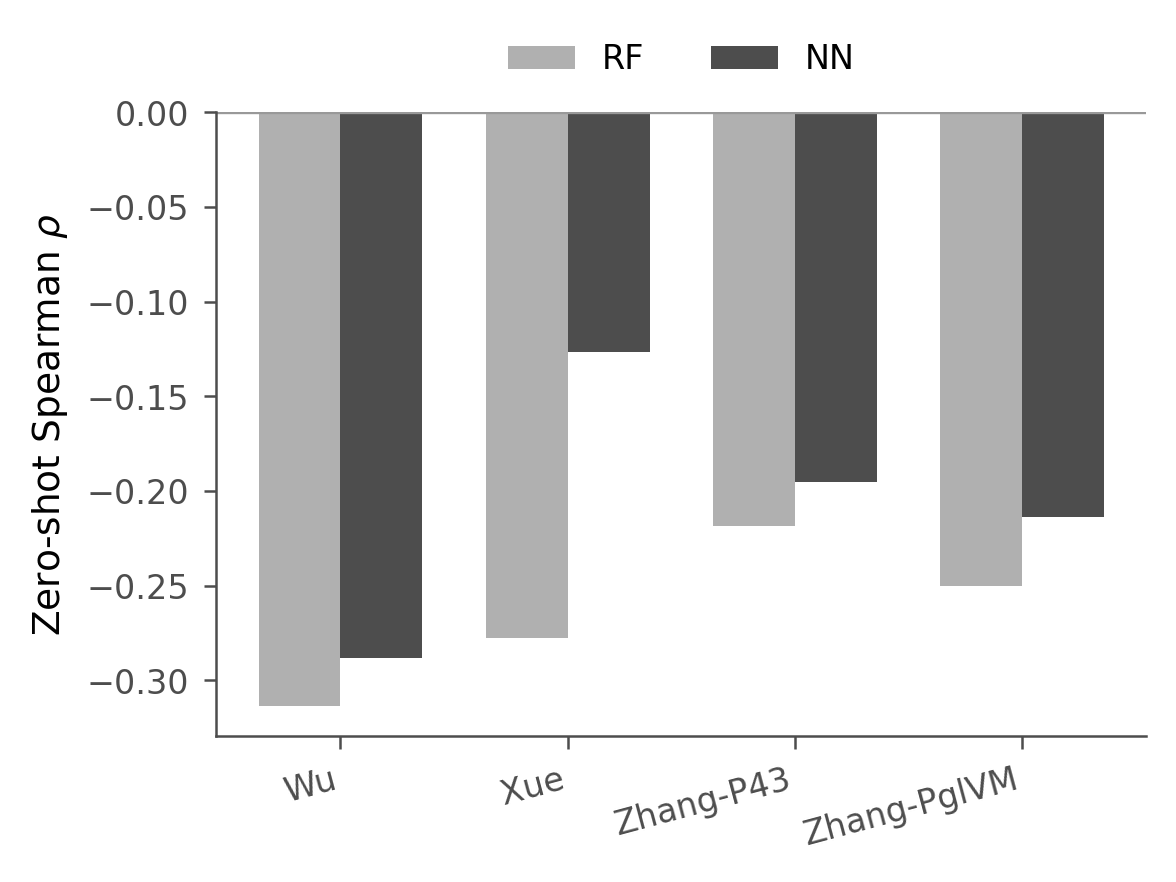
\includegraphics[width=0.62\textwidth]{../figures/cross_dataset_generalization.png}
    \caption{Cross-dataset generalization results. Zero-shot Spearman correlations between predicted and observed signal peptide efficiency across four external datasets, for the random forest (RF) and neural network (NN). All correlations are negative; per-dataset $p$-values are given in Table~\ref{tab:cross}.}
    \label{fig:cross}
\end{figure}

\paragraph{Fine-tuning results.}
Given the uniformly negative zero-shot correlations, we next test whether fine-tuning
the pretrained vector ensemble can recover positive transfer.
Table~\ref{tab:finetune} compares zero-shot and fine-tuned performance of the ESM2-650M
vector regression ensemble on each external dataset; the zero-shot values differ from
Table~\ref{tab:cross} because they come from the vector ensemble rather than the scalar RF/NN models.

\begin{table}[H]
\centering
\caption{Cross-dataset fine-tuning results. The pretrained vector regression ensemble is
fine-tuned on each external dataset using 5-fold CV $\times$ 5 seeds. Zero-shot uses the
vector model directly; fine-tuned replaces and retrains the output head. Both correlations
are computed as a single \emph{pooled out-of-fold} Spearman $\rho$ over all held-out
predictions, with a 5000-resample bootstrap 95\% CI; significance is judged by whether the
CI excludes zero. (This corrects an earlier mean-of-per-fold estimator, which is upward-biased
in magnitude and had masked the Wu effect.)}
\label{tab:finetune}
\begin{tabular}{lrcc}
\toprule
Dataset & $N$ & Zero-Shot $\rho$ & Fine-Tuned $\rho$ [95\% CI] \\
\midrule
Wu (binary) & 81 & $-$0.227 & $+$0.341 [$+$0.131, $+$0.536] \\
Xue & 322 & $-$0.104 & $-$0.192 [$-$0.296, $-$0.086] \\
Zhang-P43 & 114 & $-$0.194 & $-$0.316 [$-$0.479, $-$0.133] \\
Zhang-PglVM & 114 & $-$0.269 & $-$0.231 [$-$0.398, $-$0.051] \\
\bottomrule
\end{tabular}
\end{table}

On the pooled out-of-fold estimate, fine-tuning \emph{significantly} reverses the negative
zero-shot correlation for the binary Wu dataset, shifting Spearman $\rho$ from $-$0.227 to
$+$0.341 with a 95\% CI of [$+$0.131, $+$0.536] that excludes zero. For the three continuous
datasets, fine-tuning instead \emph{significantly worsens} the (already negative) correlations:
Xue $-$0.104 $\to$ $-$0.192, Zhang-P43 $-$0.194 $\to$ $-$0.316, Zhang-PglVM $-$0.269 $\to$ $-$0.231,
all with CIs excluding zero on the negative side.
The deterioration likely reflects overfitting of the fine-tuned output head to spurious
correlations in the small training folds (64--258 samples per fold),
compounded by the fundamental biological differences between the Grasso and external experimental systems.
So fine-tuning helps only the binary task and hurts the continuous ones; PLM representations
do not transfer secretion-efficiency \emph{magnitude} across these systems.
Figure~\ref{fig:finetune} visualizes the zero-shot versus fine-tuned performance.

\begin{figure}[H]
    \centering
    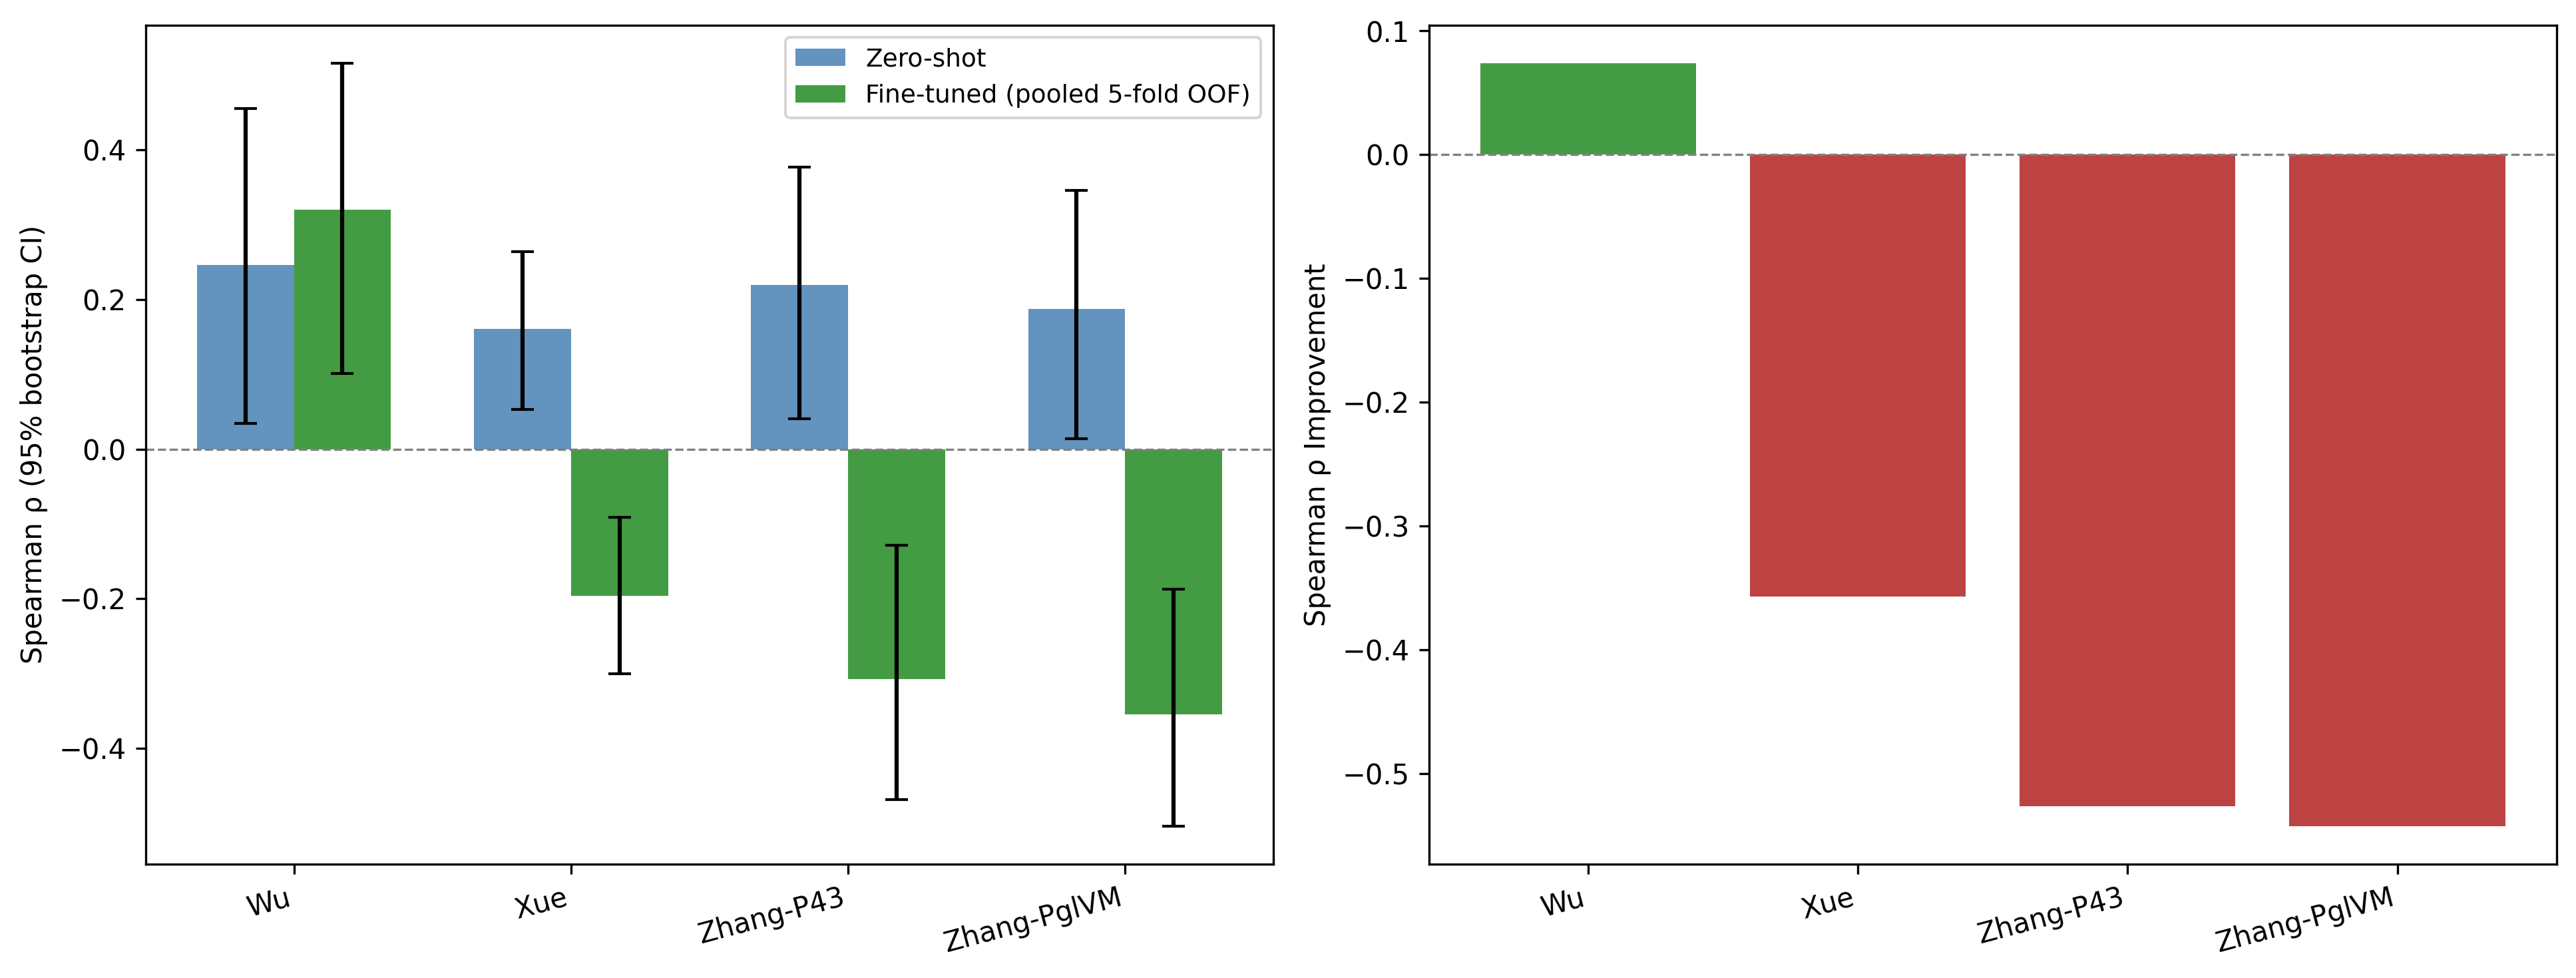
\includegraphics[width=0.62\textwidth]{../figures/cross_dataset_finetuning.png}
    \caption{Cross-dataset fine-tuning results. Zero-shot vs.\ fine-tuned pooled out-of-fold
    Spearman correlations for the vector regression ensemble on four external datasets. Error
    bars are 95\% bootstrap confidence intervals on the pooled estimate.}
    \label{fig:finetune}
\end{figure}

\subsection{Design Task Evaluation}
\label{sec:design_results}

Beyond generalization to external datasets, we also evaluate whether the models can guide the design of new signal peptide variants within the Grasso system.
Table~\ref{tab:design} summarizes model performance on ranking 4832 designed signal peptide variants across 131 genes (of 134 total, after requiring $\geq$5 variants per gene).

\begin{table}[H]
\centering
\caption{Design task evaluation across two feature representations ($N = 4832$ variants across 131 genes). Models predict relative performance of designed signal peptide variants compared to wild type.}
\label{tab:design}
\begin{tabular}{llcccc}
\toprule
Features & Model & Spearman $\rho$ & Pearson $r$ & MSE & ClassAcc (\%) \\
\midrule
ESM2-650M (1280d) & NN & \textbf{0.390} & \textbf{0.403} & 4.05 & 72.0 \\
PhysChem (156d) & NN & 0.378 & 0.388 & \textbf{4.02} & 72.5 \\
PhysChem (156d) & RF & 0.369 & 0.378 & 4.07 & \textbf{74.2} \\
ESM2-650M (1280d) & RF & 0.363 & 0.367 & 4.15 & 72.9 \\
\bottomrule
\end{tabular}
\end{table}

All four models achieve Spearman correlations above 0.36 and classification accuracy above 71\%, with all correlations significant at $p < 10^{-150}$.
The ESM2-650M NN achieves the highest rank correlation ($\rho = 0.390$), outperforming the PhysChem NN (0.378), PhysChem RF (0.369), and ESM2-650M RF (0.363).
RF models achieve marginally better classification accuracy (74.2\% PhysChem, 72.9\% ESM2-650M) than NNs (72.0--72.5\%).
The improvement from ESM2-650M over PhysChem features is modest for the design task, consistent with the smaller RF--NN gap observed for scalar regression (Section~\ref{sec:results}).

To compare directly with the design validation in \citet{grasso2023} (their Figure~4e: 11 of 15 designed peptides fell within $\pm 1$ WA of prediction, 73\%), we compute the fraction of designed variants whose predicted WA lands within $\pm 1$ of the measured value. All four models achieve ${\sim}41\%$ (PhysChem RF 41.1\%, PhysChem NN 41.4\%, ESM2 RF 41.3\%, ESM2 NN 40.9\%). This is lower than Grasso's 73\%, but the comparison is not apples-to-apples: their 15 designs were hand-picked and independently re-assayed in nanoliter reactors, whereas we evaluate the \emph{full} ${\sim}4{,}800$-variant library against the original (noisier) library-screening WA --- an unselected, lower-bias evaluation. The parity plot (Figure~\ref{fig:design_parity}) shows predicted versus measured WA per model.

\begin{figure}[H]
    \centering
    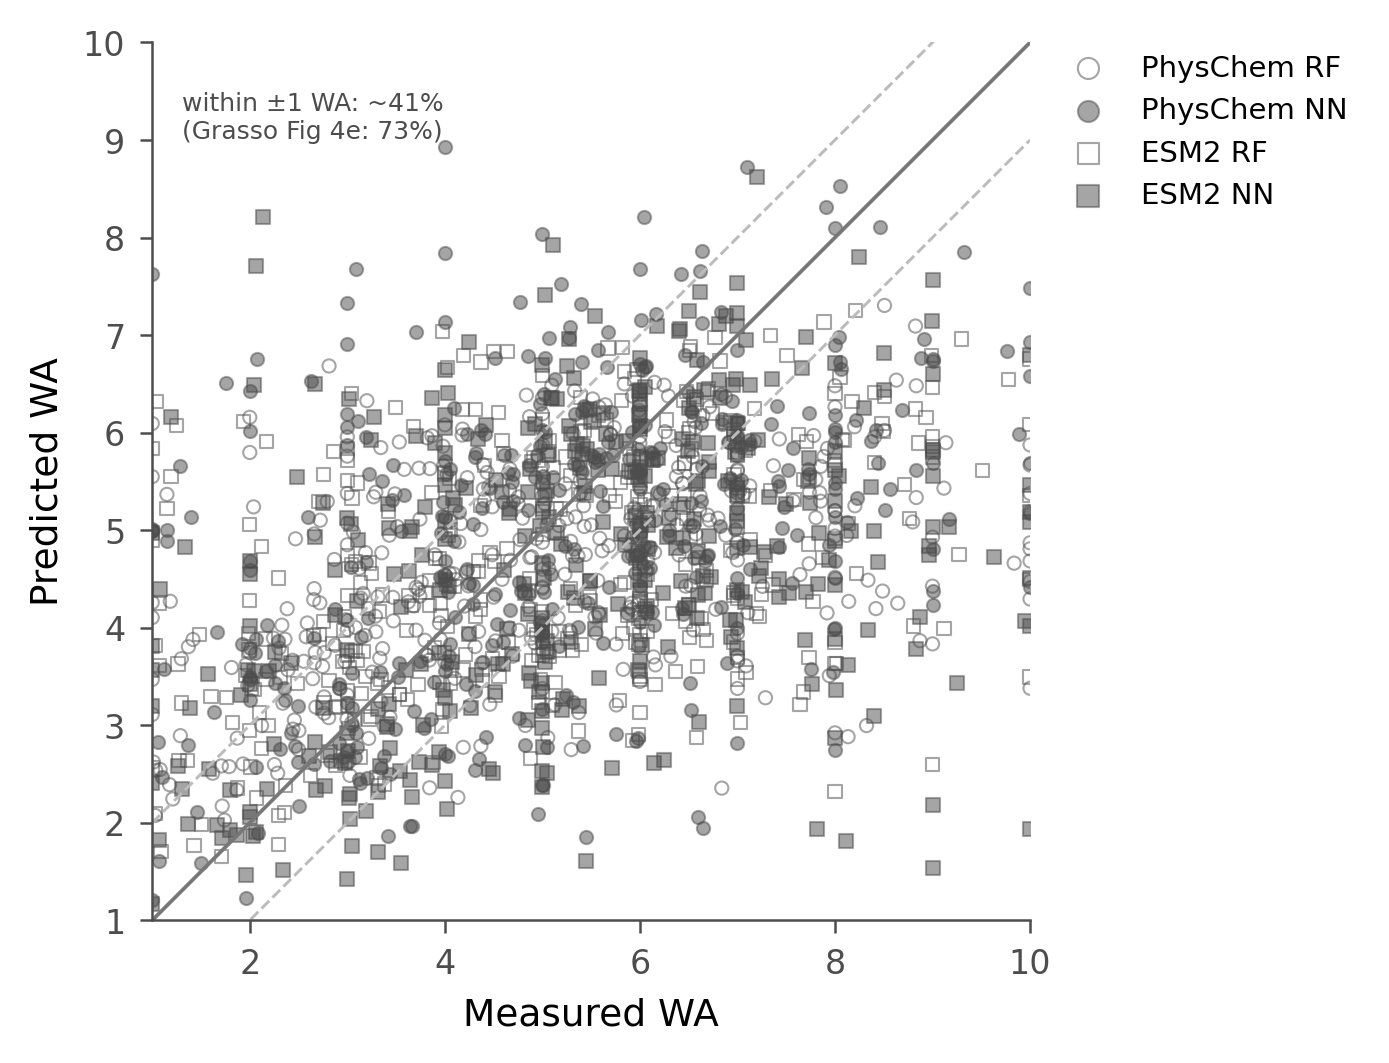
\includegraphics[width=0.55\textwidth]{../figures/design_parity.png}
    \caption{Design-task parity (predicted vs.\ measured WA) for the full design library, by featurization (PhysChem = circle, ESM2 = square) and model (RF = open, NN = filled); dashed line is $y=x$. Comparable metric to Grasso Fig.~4e: ${\sim}41\%$ of variants fall within $\pm 1$ WA (vs.\ their 11/15 = 73\% on 15 curated, independently re-assayed designs).}
    \label{fig:design_parity}
\end{figure}

% ══════════════════════════════════════════════════════════════════════════
\section{Discussion}
\label{sec:discussion}

\begin{table}[H]
\centering
\small
\caption{Summary of key results.}
\label{tab:summary}
\resizebox{\textwidth}{!}{%
\begin{tabular}{lrl}
\toprule
Result & Value & Reference \\
\midrule
\textbf{Reproducible headline: open-weight ensemble MSE} & $\mathbf{0.981 \pm 0.005}$ & Table~\ref{tab:open_ensemble} \\
\quad Improvement over baseline (1.22) & ${\sim}20\%$ & Table~\ref{tab:open_ensemble} \\
ESM2-650M single-embedding MSE (open) & $1.072 \pm 0.006$ & Table~\ref{tab:open_ensemble} \\
Ginkgo AA-0 (best, but API discontinued) & $0.959 \pm 0.014$ & Table~\ref{tab:open_ensemble} \\
Reproducible AA-0 vector NN (mean $\pm$ std) & $0.957 \pm 0.009$ & Table~\ref{tab:fulldata} \\
Linear probe MSE (vs.\ NN) & 1.037 (most of improvement) & Table~\ref{tab:baselines} \\
LOGO CV MSE (realistic generalization) & 2.19 (Spearman 0.72) & Section~\ref{sec:gene_stratified} \\
Design task Spearman $\rho$ & 0.363--0.390 & Table~\ref{tab:design} \\
\bottomrule
\end{tabular}}
\end{table}

\paragraph{Model--Representation Interaction.}
The interaction between model type and feature representation (Table~\ref{tab:comparison}) likely reflects a fundamental difference in how RF and NN handle high-dimensional inputs.
RF's random subspace sampling provides robustness to uninformative dimensions but limits its ability to exploit complex feature interactions, explaining why it plateaus across all four feature sets.
Neural networks can learn nonlinear combinations of PLM embedding dimensions that capture secretion-relevant information, but require sufficient input richness to outperform simpler methods.
The poor NN performance on physicochemical features (MSE 1.328) likely reflects a dimensionality mismatch: with only 156 input dimensions and $\sim$3000 training samples, the neural network cannot learn useful representations beyond what RF already captures through axis-aligned splits, and the higher capacity becomes a liability rather than an asset.

\paragraph{PLM Model Size.}
A related question is whether larger PLMs automatically produce better predictions.
Surprisingly, the largest PLM (ESM2-3B, 2560 dimensions) does not yield the best results.
For RF, ESM2-3B performs worst among all models.
For NN, ESM2-3B (MSE 1.067) outperforms ESM2-650M (1.090) but is still outperformed by Ginkgo-AA0 (1.050).
With only $\sim$3000 training samples, the additional dimensions of the 3B model may introduce noise without proportional signal.
The Ginkgo-AA0 model, despite having fewer parameters than ESM2-3B, may encode more task-relevant biological information for signal peptide function.

\paragraph{Vector Regression.}
Beyond the choice of input features, the regression formulation itself also matters.
Predicting bin probability distributions instead of scalar WA values yields a 4.7\% MSE improvement over the best scalar NN (1.050 $\to$ 1.001).
This gain likely arises from the richer supervision signal: each training example provides 10 target values instead of one, and the softmax output naturally enforces a valid probability distribution.
Focal loss provides a marginal improvement over cross-entropy (+2.3\% MSE; Section~\ref{sec:output_formulation}), and a controlled comparison across five output formulations confirms that the gain comes primarily from predicting 10-bin distributions rather than from the loss function: the 10-bin CCE model (MSE 0.994) outperforms all classification baselines (MSE 1.13--1.29).
However, the vector and scalar NNs also differ in activation function (LeakyReLU vs.\ ReLU) and the absence of batch normalization (Appendix~\ref{app:relu_squared}), so the improvement cannot be attributed solely to the distributional output without further ablation.
With an 80/20 validation split, the best vector model achieves MSE 1.001 --- already an 18\% improvement over the published baseline of 1.22.
The reproducible vector-NN result on Ginkgo AA-0, reported as a mean over independent retrains, is ${\sim}0.96$--$0.98$ (e.g.\ $0.957 \pm 0.009$ at dropout 0.35), a ${\sim}19$--$21\%$ improvement over the baseline (Section~\ref{sec:fulldata_results}).
The key ingredients are (i) an additional hidden layer providing greater model capacity, (ii) dropout regularization, and (iii) multi-seed ensembling to reduce prediction variance.
We stress that the reproducible contribution is methodological as much as numerical: the most reliable single intervention is ensembling, which reduces the ${\sim}{\pm}0.05$ per-model seed variance.

\paragraph{Reproducibility and high variance (a cautionary example).}
\label{sec:repro}
The single most important lesson of this work is that the vector-regression architecture is inherently high-variance --- ${\sim}{\pm}0.05$ MSE per single model --- so any single un-replicated number is unreliable, and all performance must be reported as a mean $\pm$ standard deviation over independent retrains with bootstrap confidence intervals.
A reproducibility audit established this concretely. An earlier headline of ``MSE 0.932'' for the (256, 256, 128)/dropout-0.35 configuration \emph{did not reproduce}: re-training the identical configuration gives $0.957 \pm 0.009$ (dropout 0.35) or $0.978 \pm 0.012$ (dropout 0.20), and 0.932 was never recovered in 10 retrains --- it was a favorable tail draw below the minimum of either distribution.
A prior Wolfram-language single-model benchmark of 0.953 is likewise a favorable draw: running its original code across 8 random seeds gives $0.99 \pm 0.046$ (range [0.94, 1.07]), with 0.953 sitting ${\sim}0.8$ standard deviations below the mean. Both ``benchmarks'' are seed noise of the same ${\sim}0.97$--$0.99$ distribution; neither is a stable number to beat.
This reframes the honest headline: the reproducible vector-NN result is ${\sim}0.96$--$0.99$ over seeds, a ${\sim}19$--$21\%$ improvement over the random forest baseline (1.22), and the demonstration that earlier single-draw ``benchmarks'' were not reproducible is itself a substantive methodological finding.
A related corrected practice concerns hyperparameter selection: the earlier dropout of 0.35 was selected on test-set MSE, which is a repudiated practice. On a held-out validation split, all dropout values in 0.20--0.35 are statistically indistinguishable (Appendix~\ref{app:dropout_val}), so we report the validation-selected configuration and treat the previous test-set selection as a corrected limitation.

\paragraph{A reproducible open-weight headline.}
The best single embedding in our experiments is Ginkgo AA-0 ($0.959 \pm 0.014$), but it is API-only, proprietary, and the API has been discontinued: its embeddings can no longer be regenerated by anyone, so basing the central claim on AA-0 would rest it on a permanently unreproducible input.
We therefore anchor the headline on open weights. An ensemble of architecturally diverse open PLMs --- ProtT5, ESM2-650M, and ProtBERT --- achieves $0.981 \pm 0.005$ (Table~\ref{tab:open_ensemble}), recovering all but ${\sim}0.02$ of AA-0's performance while remaining fully reproducible from public HuggingFace checkpoints, and improving ${\sim}20\%$ over the Grasso baseline.
The ensemble pays off because the three open models are quality-comparable (ProtT5 1.017, ESM2-650M 1.072, ProtBERT 1.084), so averaging their decorrelated errors yields a real gain; ensembling AA-0 with ESM2 \emph{failed} precisely because the dominant AA-0 diluted into the weaker model. A linear probe confirms AA-0 and ESM2-650M encode essentially the same signal (Pearson $r = 0.975$), so the open ensemble recovers AA-0's information, not merely its score.

\paragraph{Cross-Dataset Generalization.}
The cross-dataset results carry a stark practical implication: naively applying a signal peptide model trained in one system to another is not merely unhelpful but actively misleading.
All four external datasets show negative Spearman correlations, meaning that sequences the model predicts as high-performing tend to perform worst in the new context.
This likely reflects host- or cargo-specific signal patterns learned from the Grasso data that are maladaptive elsewhere, since signal peptide efficiency depends on the cargo protein, promoter, host organism, and growth conditions.
A signal peptide optimized for $\alpha$-amylase secretion in \textit{B.\ subtilis} may be poorly suited for xylanase production in the same organism, let alone for enzyme secretion in \textit{E.\ coli} or \textit{S.\ cerevisiae}.
The Zhang cross-promoter analysis provides complementary evidence: the same 114 signal peptides correlate at $r = 0.977$ across two promoters, confirming that signal peptide rankings are partially conserved within a system but not across systems.
In practice, this means models for signal peptide optimization need to be trained on task-specific data rather than transferred across experimental contexts.
Fine-tuning the pretrained vector ensemble on target-domain data helps only the binary task:
freezing the learned feature layers and retraining only the output head \emph{significantly}
reverses the negative correlation for Wu ($-$0.227 $\to$ $+$0.341, 95\% CI [$+$0.131, $+$0.536]),
the sole binary-outcome dataset, but significantly \emph{worsens} the three continuous datasets
(Xue: $-$0.104 $\to$ $-$0.192; Zhang-P43: $-$0.194 $\to$ $-$0.316; Zhang-PglVM: $-$0.269 $\to$ $-$0.231,
all CIs excluding zero). Wu's binary labels are evidently easier to learn from limited data than
continuous activity magnitudes, which do not transfer across these experimental systems.
These results underscore that transfer learning for signal peptide efficiency remains
severely data-limited, and that fine-tuning on small datasets risks overfitting rather than recovering
transferable patterns.

\paragraph{Design Task.}
Despite the limited cross-dataset transferability, the models still prove useful within the Grasso experimental system.
The design task demonstrates that models trained on characterized variants can meaningfully rank novel designed signal peptides, with Spearman $\rho = 0.36$--0.39 and classification accuracy of 72--74\%, well above the 50\% random baseline.
Generating ESM2-650M embeddings for the design variants and evaluating all four model--feature combinations reveals that the ESM2-650M NN achieves the highest rank correlation ($\rho = 0.390$), though the improvement over PhysChem features is modest (0.390 vs.\ 0.378 for NN, 0.363 vs.\ 0.369 for RF).
This contrasts with the larger PLM advantage observed in the scalar regression task, suggesting that the design task's evaluation structure (per-gene ranking rather than absolute WA prediction) may limit the benefit of richer representations.
The moderate but significant correlations suggest that these models can serve as a practical filter for prioritizing candidates in experimental screening campaigns.

\paragraph{Limitations.}
Several methodological caveats apply.
The RF and NN hyperparameter searches used different validation strategies (5-fold CV vs.\ single train/val split), which may introduce some asymmetry in the comparison.
The full-data optimized models train without a validation split, which precludes early stopping; we compensate with dropout and ensembling.
We note as a corrected limitation that an earlier version of this work selected the dropout of 0.35 based on test-set MSE, which is a repudiated practice; we now report the validation-selected configuration.
Appendix~\ref{app:dropout_val} shows that all dropout values $\geq 0.20$ produce statistically indistinguishable validation MSE.
The external fine-tuning datasets are small (81--322 sequences), so even the pooled out-of-fold correlations we report carry wide bootstrap intervals; the cross-dataset conclusions should be read as directional rather than precise.
Validation MSE improves from 1.375 at dropout 0.15 to 1.333--1.347 for all dropout rates $\geq 0.20$, with no statistically significant differences among them (all within seed-to-seed variability of $\pm$0.07--0.09); the test-optimal dropout (0.35) produces a validation MSE of 1.347 $\pm$ 0.072, indistinguishable from the validation-optimal (0.20, MSE 1.333 $\pm$ 0.084).
The differences between top-performing models are modest; 95\% bootstrap confidence intervals for all models are reported in Appendix~\ref{app:bootstrap}.
The cross-dataset significance tests (Table~\ref{tab:cross}) involve eight comparisons; after Bonferroni correction ($\alpha = 0.00625$), all four NN correlations and two of the four RF correlations no longer reach significance. Only the Wu and Xue RF correlations survive correction.

In terms of scope, the dataset is limited to \textit{B.\ subtilis} with a single reporter enzyme.
Ginkgo-AA0 embeddings yield the best single-embedding result but are derived from a proprietary, now-discontinued model and are permanently unreproducible; the reproducible open-weight ensemble (ProtT5 + ESM2-650M + ProtBERT, $0.981 \pm 0.005$) recovers all but ${\sim}0.02$ of that performance, confirming that the central result is not contingent on proprietary representations.
Cross-dataset and fine-tuning evaluations use ESM2-650M embeddings (open and reproducible), so the transferability of the discontinued Ginkgo-AA0 representations specifically remains untested.
The vector regression architecture uses LeakyReLU activation, omits batch normalization, and does not apply L2 kernel regularization,
while the scalar NN uses ReLU with batch normalization and L2 regularization; a systematic ablation of these
architectural differences was not performed, so the vector regression improvement cannot
be attributed solely to the distributional output.
The original Grasso train/test partition contains overlapping genes (132 of 134 genes appear in both sets), meaning the model may partly learn gene-specific patterns rather than generalizable signal peptide features.
A leave-one-gene-out cross-validation (Section~\ref{sec:gene_stratified}) addresses this concern.

% ══════════════════════════════════════════════════════════════════════════
\section{Conclusion}
\label{sec:conclusion}

We have systematically evaluated signal peptide efficiency prediction across multiple feature representations, two model architectures, and two regression formulations, with additional analyses that probe the sources --- and the reproducibility --- of predictive performance.
A vector regression neural network with PLM embeddings and focal loss, combined with multi-seed ensembling, substantially improves over the random forest baseline.
Our reproducible headline is an ensemble of architecturally diverse \emph{open-weight} PLMs (ProtT5, ESM2-650M, ProtBERT) achieving a test MSE of $0.981 \pm 0.005$ (mean $\pm$ std over independent retrains), a ${\sim}20\%$ improvement over the published baseline of 1.22 and recoverable by anyone from public model weights.
The best single embedding, the proprietary Ginkgo AA-0 ($0.959 \pm 0.014$), is marginally stronger but its API has been discontinued and its embeddings can no longer be regenerated, so we report it only as a caveated historical comparison; a linear probe shows AA-0 and ESM2-650M capture essentially the same signal (Pearson $r = 0.975$).
Because this architecture is high-variance (${\sim}{\pm}0.05$ per single model), we report every number as a mean $\pm$ standard deviation with bootstrap CIs; an earlier ``0.932'' headline and a prior ``0.953'' benchmark were both shown to be non-reproducible favorable seed draws of the same ${\sim}0.97$--$0.99$ distribution.

Two findings temper these results.
First, a linear probe (single Dense layer) on the same embeddings achieves MSE near the full network, indicating that the PLM embedding encodes the majority of task-relevant information; the MLP architecture contributes a modest further refinement.
Second, leave-one-gene-out cross-validation yields MSE 2.19 (Spearman $\rho = 0.720$), a sharp increase over the standard split, reported as the realistic cross-gene generalization metric (132 of 134 genes overlap train and test in the standard split, inflating apparent performance).
The model retains meaningful cross-gene predictive ability ($\rho = 0.720$), but future evaluations should use gene-stratified splits to provide realistic generalization estimates.

Cross-dataset evaluation reveals that zero-shot predictions do not generalize across organisms or experimental systems; on pooled out-of-fold statistics, fine-tuning the output head significantly reverses the negative correlation for the binary Wu dataset (Spearman $\rho$ from $-$0.227 to $+$0.341, 95\% CI [$+$0.131, $+$0.536]) but significantly worsens the three continuous datasets, so secretion-efficiency magnitude does not transfer across these systems.
Applied to designed variants, the models achieve classification accuracy of 72--74\% and Spearman $\rho$ up to 0.390, demonstrating practical utility for guiding experimental prioritization within the training domain.

Random forests remain competitive and robust across feature types, making them suitable when interpretability or computational efficiency is prioritized.
These results demonstrate that PLM embeddings encode rich biological information for signal peptide prediction, but that standard evaluation protocols can substantially overestimate generalization; gene-stratified cross-validation provides a more realistic assessment of model utility.
Future work could explore end-to-end fine-tuning of PLM weights on secretion efficiency data, region-aware embedding pooling strategies, or extending the analysis to additional host organisms and cargo proteins.

% ══════════════════════════════════════════════════════════════════════════
\section*{Data Availability}

The original dataset is available as supplementary material to \citet{grasso2023}.
PLM embeddings were generated using publicly available model weights.
All analysis code and results are available at \url{https://github.com/Mehak-W/signal-peptide-secretion}.

% ══════════════════════════════════════════════════════════════════════════
\bibliographystyle{unsrtnat}
\bibliography{references}

% ══════════════════════════════════════════════════════════════════════════
\appendix

% ── Appendix A: Hyperparameter Search Results ─────────────────────────────
\section{Hyperparameter Search Results}
\label{app:hyperparam}

Tables~\ref{tab:rf_trials} and \ref{tab:nn_trials} report the top-5 configurations per feature type from the randomized hyperparameter searches (100 RF configs with 5-fold CV; 40 NN configs with 80/20 validation split).
Full trial data are available in the GitHub repository.

\begin{table}[H]
\centering
\caption{Top-5 random forest configurations per feature type, ranked by 5-fold cross-validation MSE (100 configs searched per type).}
\label{tab:rf_trials}
\small
\begin{tabular}{clccccc}
\toprule
Feature & Rank & $n_{\text{est}}$ & Depth & Split & Leaf & CV MSE \\
\midrule
\multirow{5}{*}{PhysChem}
 & 1 & 75 & None & 5 & 2 & 2.019 \\
 & 2 & 50 & 25 & 2 & 1e-4 & 2.021 \\
 & 3 & 150 & 30 & 2 & 1e-4 & 2.028 \\
 & 4 & 100 & 30 & 10 & 1e-3 & 2.029 \\
 & 5 & 150 & 25 & 2 & 2 & 2.029 \\
\midrule
\multirow{5}{*}{ESM2-650M}
 & 1 & 300 & 25 & 1e-3 & 4 & 1.843 \\
 & 2 & 200 & 20 & 2 & 1e-3 & 1.845 \\
 & 3 & 300 & None & 10 & 4 & 1.845 \\
 & 4 & 75 & 25 & 5 & 1e-3 & 1.847 \\
 & 5 & 200 & 20 & 2 & 4 & 1.847 \\
\midrule
\multirow{5}{*}{ESM2-3B}
 & 1 & 150 & 25 & 2 & 2 & 1.925 \\
 & 2 & 300 & 25 & 1e-3 & 4 & 1.927 \\
 & 3 & 100 & 30 & 10 & 1e-3 & 1.928 \\
 & 4 & 200 & 25 & 2 & 1e-3 & 1.929 \\
 & 5 & 200 & 25 & 1e-3 & 1e-3 & 1.929 \\
\midrule
\multirow{5}{*}{Ginkgo-AA0}
 & 1 & 300 & None & 10 & 4 & 1.723 \\
 & 2 & 75 & None & 2 & 1e-4 & 1.723 \\
 & 3 & 150 & 30 & 2 & 1e-4 & 1.724 \\
 & 4 & 200 & 20 & 2 & 1e-3 & 1.724 \\
 & 5 & 100 & 25 & 2 & 2 & 1.725 \\
\bottomrule
\end{tabular}
\end{table}

\begin{table}[H]
\centering
\caption{Top-5 neural network configurations per feature type (non-log-transformed targets), ranked by validation MSE (40 configs searched per type, 80/20 train/val split). Log-transformed target variants were also evaluated during the search but are excluded here since the optimal skewness was below the transformation threshold (Section~\ref{sec:preprocessing}). Full trial data are available in the GitHub repository.}
\label{tab:nn_trials}
\small
\begin{tabular}{clccccr}
\toprule
Feature & Rank & Layers & Drop & L2 & LR / Batch & Val MSE \\
\midrule
\multirow{5}{*}{PhysChem}
 & 1 & 256, 128 & 0.3 & 0.01 & 1e-3 / 64 & 1.390 \\
 & 2 & 128, 64 & 0.3 & 0.01 & 1e-3 / 32 & 1.425 \\
 & 3 & 128, 64 & 0.4 & 1e-4 & 1e-3 / 64 & 1.515 \\
 & 4 & 128, 64 & 0.5 & 0.01 & 5e-4 / 64 & 1.529 \\
 & 5 & 128, 64 & 0.4 & 1e-3 & 5e-4 / 64 & 1.551 \\
\midrule
\multirow{5}{*}{ESM2-650M}
 & 1 & 256, 128 & 0.4 & 0.01 & 1e-3 / 64 & 1.241 \\
 & 2 & 256 & 0.3 & 1e-3 & 5e-4 / 64 & 1.266 \\
 & 3 & 512, 256 & 0.5 & 0.01 & 5e-4 / 64 & 1.300 \\
 & 4 & 256, 128 & 0.5 & 1e-4 & 5e-4 / 64 & 1.331 \\
 & 5 & 256, 128 & 0.4 & 0.01 & 5e-4 / 32 & 1.353 \\
\midrule
\multirow{5}{*}{ESM2-3B}
 & 1 & 1024, 512 & 0.4 & 0.01 & 1e-3 / 64 & 1.302 \\
 & 2 & 512, 256 & 0.5 & 1e-3 & 1e-3 / 32 & 1.316 \\
 & 3 & 512, 256 & 0.4 & 1e-3 & 5e-4 / 32 & 1.333 \\
 & 4 & 512, 256 & 0.3 & 1e-3 & 1e-3 / 64 & 1.377 \\
 & 5 & 512, 256 & 0.2 & 0.01 & 5e-4 / 32 & 1.387 \\
\midrule
\multirow{5}{*}{Ginkgo-AA0}
 & 1 & 256, 128 & 0.3 & 1e-4 & 5e-4 / 32 & 1.146 \\
 & 2 & 512, 256 & 0.5 & 1e-3 & 5e-4 / 64 & 1.197 \\
 & 3 & 256 & 0.2 & 1e-3 & 1e-3 / 32 & 1.224 \\
 & 4 & 256, 128 & 0.5 & 1e-4 & 1e-3 / 64 & 1.236 \\
 & 5 & 256, 128 & 0.5 & 0.01 & 1e-3 / 32 & 1.248 \\
\bottomrule
\end{tabular}
\end{table}

% ── Appendix B: Vector Regression Per-Seed Results ────────────────────────
\section{Vector Regression Per-Seed Results}
\label{app:vector_seeds}

Table~\ref{tab:vector_seeds} reports the per-seed test MSE for all six embedding--loss combinations, along with the ensemble mean.

\begin{table}[H]
\centering
\caption{Per-seed test MSE for vector regression models. Each model uses the base architecture (2$\times$256 hidden units, LeakyReLU, 20\% dropout, softmax output) with 5 random seeds for train/validation splitting.}
\label{tab:vector_seeds}
\begin{tabular}{llcccccr}
\toprule
Embedding & Loss & Seed 42 & Seed 123 & Seed 456 & Seed 789 & Seed 1024 & Ensemble \\
\midrule
Ginkgo-AA0 & Focal & 1.026 & 1.120 & 1.023 & 1.128 & 1.046 & \textbf{1.001} \\
Ginkgo-AA0 & CE & 1.053 & 1.102 & 1.054 & 1.111 & 1.050 & 1.003 \\
ESM2-650M & Focal & 1.084 & 1.158 & 1.100 & 1.169 & 1.125 & 1.049 \\
ESM2-650M & CE & 1.084 & 1.151 & 1.093 & 1.194 & 1.132 & 1.054 \\
ESM2-3B & CE & 1.235 & 1.224 & 1.179 & 1.196 & 1.214 & 1.109 \\
ESM2-3B & Focal & 1.215 & 1.220 & 1.185 & 1.226 & 1.193 & 1.117 \\
\bottomrule
\end{tabular}
\end{table}

% ── Appendix C: Architecture Search Landscape ─────────────────────────────
\section{Architecture Search Landscape}
\label{app:arch_search}

Figure~\ref{fig:arch_search} shows the full architecture search landscape from the initial full-data vector regression exploration, which identified the (256, 256, 128) three-layer architecture as the top performer prior to the dropout and ensemble optimization in Section~\ref{sec:fulldata_results}.

\begin{figure}[H]
    \centering
    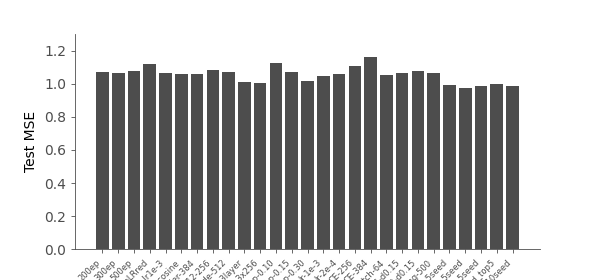
\includegraphics[width=0.95\textwidth]{../figures/vector_architecture_search.png}
    \caption{Architecture search results for full-data vector regression (Ginkgo-AA0 + focal loss). Configurations are ranked by test MSE on all 1326 test samples. The three-layer (256, 256, 128) architecture with 5-seed ensemble achieved the lowest MSE (0.973), motivating the subsequent dropout optimization (Section~\ref{sec:fulldata_results}).}
    \label{fig:arch_search}
\end{figure}

% ── Appendix D: Bootstrap Confidence Intervals ────────────────────────────
\section{Bootstrap Confidence Intervals}
\label{app:bootstrap}

To quantify uncertainty in test set performance, we compute 95\% bootstrap confidence intervals (10{,}000 resamples) for all 16 models (including the full-data optimized model).
Each model is retrained with its best configuration and evaluated on the held-out test set; the test set is then resampled with replacement to obtain the bootstrap distribution.
These CIs capture uncertainty due to finite test-set size (sampling variability) but \emph{not} model uncertainty from random initialization; for ensemble models, the ensemble prediction is fixed before bootstrapping begins.
This is an important caveat: because the architecture is high-variance across random seeds (${\sim}{\pm}0.05$ MSE; Section~\ref{sec:repro}), the dominant uncertainty for any single configuration is initialization variance, which these bootstrap CIs do not capture. The mean $\pm$ standard deviation over independent retrains reported in the main text is therefore the primary reliability indicator, with these bootstrap CIs as a complementary lower bound on uncertainty.

\begin{table}[H]
\centering
\caption{Bootstrap 95\% confidence intervals for test MSE, $R^2$, and Spearman $\rho$ across all models (10{,}000 bootstrap resamples). $^\dagger$Full-data model: (256, 256, 128) architecture, dropout 0.35, trained on all 3068 samples without validation split, evaluated on all 1326 test samples. \textit{Note:} This 0.932 entry is a single un-replicated draw that does not reproduce --- re-running the identical configuration gives $0.957 \pm 0.009$ (Section~\ref{sec:repro}); it is retained here only as the historical bootstrap entry, and the bootstrap CI (which omits initialization variance) understates its true uncertainty. Point estimates may differ from the main tables because the bootstrap procedure retrains each model with a single random initialization.}
\label{tab:bootstrap}
\small
\setlength{\tabcolsep}{4pt}
\begin{tabular}{lcccccr}
\toprule
Model & MSE & 95\% CI & $R^2$ & 95\% CI & Spearman & 95\% CI \\
\midrule
\multicolumn{7}{l}{\textit{Random Forest}} \\
RF PhysChem (base) & 1.193 & [1.078, 1.317] & 0.750 & [0.724, 0.773] & 0.859 & [0.844, 0.872] \\
RF PhysChem (tuned) & 1.208 & [1.094, 1.328] & 0.747 & [0.721, 0.770] & 0.857 & [0.843, 0.870] \\
RF ESM2-650M & 1.189 & [1.076, 1.310] & 0.750 & [0.725, 0.773] & 0.853 & [0.837, 0.867] \\
RF ESM2-3B & 1.245 & [1.126, 1.366] & 0.739 & [0.713, 0.763] & 0.849 & [0.833, 0.862] \\
RF Ginkgo-AA0 & 1.158 & [1.043, 1.281] & 0.757 & [0.731, 0.781] & 0.857 & [0.841, 0.870] \\
\midrule
\multicolumn{7}{l}{\textit{Neural Network (scalar)}} \\
NN PhysChem & 1.413 & [1.253, 1.582] & 0.703 & [0.666, 0.738] & 0.828 & [0.809, 0.846] \\
NN ESM2-650M & 1.109 & [0.988, 1.240] & 0.767 & [0.738, 0.794] & 0.855 & [0.840, 0.869] \\
NN ESM2-3B & 1.175 & [1.051, 1.302] & 0.753 & [0.725, 0.780] & 0.850 & [0.835, 0.864] \\
NN Ginkgo-AA0 & 1.191 & [1.076, 1.317] & 0.750 & [0.723, 0.774] & 0.848 & [0.833, 0.861] \\
\midrule
\multicolumn{7}{l}{\textit{Vector regression (5-seed ensemble)}} \\
Vec ESM2-650M CE & 1.051 & [0.937, 1.175] & 0.780 & [0.753, 0.804] & 0.861 & [0.845, 0.875] \\
Vec ESM2-650M focal & 1.045 & [0.934, 1.167] & 0.781 & [0.755, 0.804] & 0.860 & [0.844, 0.874] \\
Vec ESM2-3B CE & 1.122 & [1.007, 1.247] & 0.765 & [0.737, 0.789] & 0.857 & [0.841, 0.870] \\
Vec ESM2-3B focal & 1.091 & [0.981, 1.211] & 0.771 & [0.745, 0.794] & 0.859 & [0.844, 0.872] \\
Vec Ginkgo-AA0 CE & 0.995 & [0.887, 1.112] & 0.791 & [0.766, 0.814] & 0.867 & [0.852, 0.880] \\
Vec Ginkgo-AA0 focal & 0.997 & [0.887, 1.115] & 0.791 & [0.765, 0.814] & 0.866 & [0.850, 0.880] \\
\midrule
\multicolumn{7}{l}{\textit{Full-data optimized (5-seed ensemble, no val split)}} \\
Vec Ginkgo-AA0 focal$^\dagger$ & 0.932 & [0.823, 1.054] & 0.804 & [0.779, 0.828] & 0.873 & [0.857, 0.887] \\
\bottomrule
\end{tabular}
\end{table}

Figure~\ref{fig:forest_plot} presents these intervals as a forest plot, showing the relative performance and uncertainty of all 16 models.

\begin{figure}[H]
    \centering
    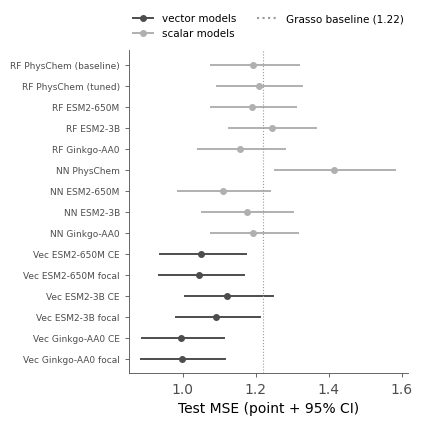
\includegraphics[width=0.6\textwidth]{../figures/bootstrap_forest_plot.png}
    \caption{Forest plot of test MSE with 95\% bootstrap confidence intervals for all 16 models. Light-gray markers indicate scalar models (RF and NN); dark-gray markers indicate vector regression ensembles. The dotted line marks the Grasso physicochemical baseline (MSE 1.22). These CIs omit initialization variance and so understate uncertainty for the high-variance vector models (Section~\ref{sec:repro}).}
    \label{fig:forest_plot}
\end{figure}

% ── Appendix E: Dropout Validation ─────────────────────────────────────────
\section{Dropout Validation}
\label{app:dropout_val}

To confirm that the dropout selection in Section~\ref{sec:fulldata_results} is not an artifact of test-set model selection, we repeated the dropout sweep using an independent 80/20 train/validation split from the training data.
For each dropout rate in $\{0.15, 0.20, 0.25, 0.30, 0.35\}$, we trained 5-seed ensembles on 80\% of the training data and evaluated on the held-out 20\% validation set.
The same (256, 256, 128) architecture, focal loss, and training protocol from Section~\ref{sec:fulldata_results} were used.

\begin{figure}[H]
    \centering
    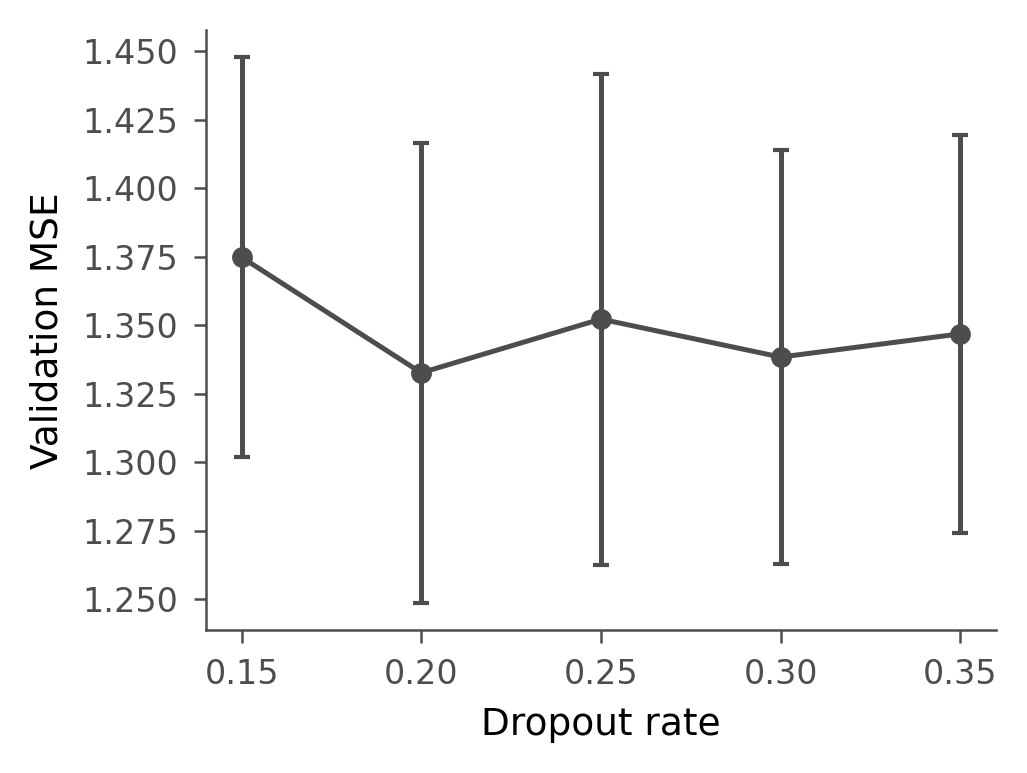
\includegraphics[width=0.75\textwidth]{../figures/dropout_validation.png}
    \caption{Dropout validation: MSE on held-out validation data (80/20 split) across dropout rates. The validation curve is essentially flat for dropout $\geq 0.20$, so the test-selected 0.35 and the validation-optimal 0.20 are statistically indistinguishable. Error bars represent standard deviation across 5 seeds. Absolute validation MSE is higher than test MSE because models train on only 80\% of the data.}
    \label{fig:dropout_val}
\end{figure}

As shown in Figure~\ref{fig:dropout_val}, validation MSE drops from 1.375 at dropout 0.15 to a minimum of 1.333 at dropout 0.20, then remains between 1.338 and 1.352 for dropout 0.25--0.35; all values at dropout $\geq 0.20$ are within seed-to-seed variability ($\pm$0.07--0.09).
The test-optimal dropout (0.35, validation MSE 1.347 $\pm$ 0.072) and the validation-optimal (0.20, 1.333 $\pm$ 0.084) are statistically indistinguishable, as are all intermediate values.
This supports the conclusion that dropout values in the range 0.20--0.35 produce equivalent generalization performance, and the test-optimal choice of 0.35 is not contradicted by the validation data.
The higher absolute MSE on validation (${}\sim$1.35 vs.\ ${}\sim$0.93 on test) is expected because validation models train on only 80\% of the data (2454 vs.\ 3068 samples).

% ── Appendix F: ReLU-Squared Activation Comparison ─────────────────────────
\section{ReLU-Squared Activation Comparison}
\label{app:relu_squared}

We compared ReLU-squared ($\text{ReLU}^2(x) = \max(0, x)^2$) against the default LeakyReLU activation in the best vector regression architecture (256, 256, 128; dropout 0.35; focal loss; 5-seed ensemble).
LeakyReLU achieves MSE 0.961 [0.847, 1.085], while ReLU-squared achieves MSE 5.11 [4.78, 5.44], a catastrophic degradation ($R^2 = -0.073$) worse than a mean-prediction baseline (MSE 4.76).
The large per-seed variance (4.67--9.07) indicates training instability rather than a systematic accuracy--sparsity tradeoff.
ReLU-squared does produce substantially sparser internal representations (Hoyer sparsity 0.67--0.92 and 56--75\% exact zeros vs.\ 0.27--0.32 and 0\% zeros for LeakyReLU), but this comes at the cost of model collapse rather than a graceful tradeoff.
This experiment uses only two learning rates (5$\times$10$^{-4}$ with fallback to 2$\times$10$^{-4}$) and does not include BatchNorm, gradient clipping, or standard ReLU controls; the catastrophic failure may therefore reflect a hyperparameter mismatch rather than a fundamental limitation of ReLU-squared.
Figure~\ref{fig:relu_sq} shows the comparison.

\begin{figure}[H]
    \centering
    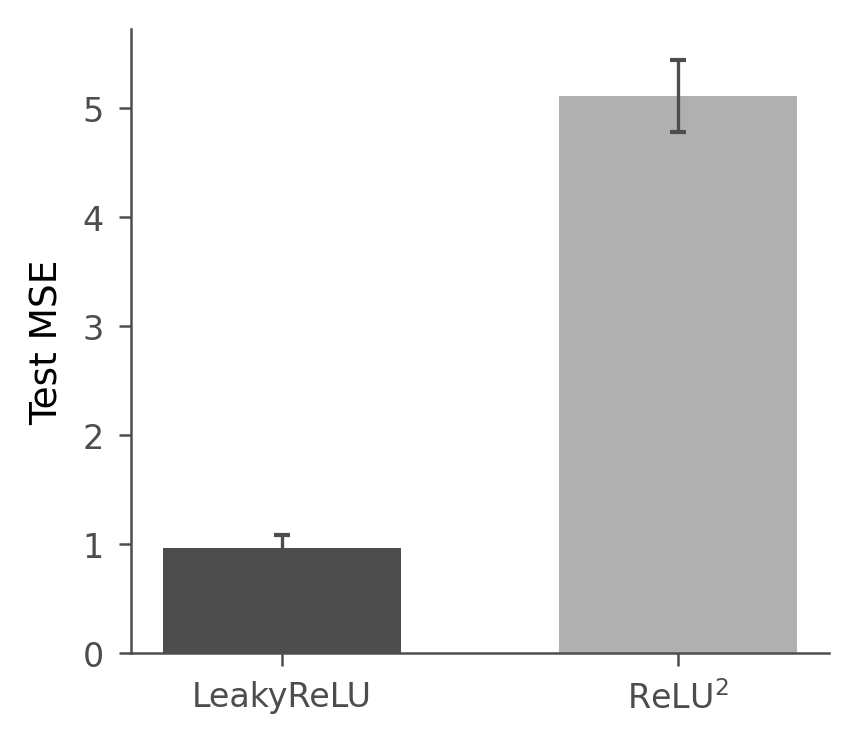
\includegraphics[width=0.5\textwidth]{../figures/relu_squared_comparison.png}
    \caption{Test MSE for LeakyReLU versus ReLU-squared activation in the vector regression architecture (256, 256, 128; dropout 0.35; focal loss; 5-seed ensemble). ReLU-squared catastrophically degrades accuracy (MSE 0.961 $\to$ 5.11) despite producing 2--3$\times$ sparser internal representations (Hoyer sparsity, discussed in text); error bars are standard deviation across 5 seeds.}
    \label{fig:relu_sq}
\end{figure}

\end{document}
